\documentclass{Vorlage}
%\usepackage[ngerman]{babel}
\usepackage{amsfonts}
\usepackage{graphicx}
\usepackage{url}
\usepackage{amsmath}
\usepackage{adjustbox}
\usepackage{color}
\usepackage{multirow}
\usepackage{bm}
%\usepackage[utf8]{inputenc}
%\bibliographystyle{apalike}
\setlength{\parindent}{0pt}

\pagestyle{fancy}
\renewcommand*\sectionmark[1]{\markboth{\MakeUppercase{#1}}{}}
\begin{document}

\newgeometry{top=2.5cm,bottom=2.0cm,left=2.5cm,right=2.5cm} % Befehl wird nur benötigt, falls Änderungen an den Seitenrändern in der Datei "Vorlage.cls" vorgenommen werden.

\begin{titlepage}

\begin{figure}
 \begin{center}
 
\includegraphics[scale=0.8]{Pictures/logo3}
 \end{center}
\end{figure}
\vspace*{3cm}




\titel{Kleinräumige Extrapolation von Umfragedaten}{}

\vspace{1cm}

\begin{tabular}{p{3.5cm}|p{0.1cm} p{10cm}l}
\textsc{Namen:} & & \textsc{Alexander Lange, Kai Husmann}\\
\textsc{Matr. Nr.:} & & \textsc{21426614, 20707176}\\
\textsc{Studiengang:} & & \textsc{Angewandte Statistik}\\
\textsc{Mail:} & & \textsc{Alexander.lange$ @ $uni-goettingen.de}\\
\textsc{} & & \textsc{Kai.Husmann$ @ $forst.uni-goettingen.de}\\
\textsc{Kurs:} & & \textsc{Statistisches Praktikum}\\
\textsc{Kursleiter:} & & \textsc{Prof.Dr. Thomas Kneib}\\
\textsc{Lehrstuhl:} & & \textsc{Statistik}\\
\textsc{Fakultät:} & & \textsc{Wirtschaftswissenschaften}\\
\textsc{Abgabedatum:} & & \textsc{30. September 2016}\\
\end{tabular}
\end{titlepage}

\restoregeometry

\pagenumbering{Roman} % \pagenumbering{roman} = Kleinschreibung: II -> ii.

\pagestyle{plain}

\tableofcontents % Inhaltsverzeichnis.

\newpage % Neue Seite.

\listoffigures % Abbildungsverzeichnis.

\listoftables % Tabellenverzeichnis.

\newpage

\pagenumbering{arabic} % Ab hier folgt die arabische Seitennummerierung.

%\renewcommand{\thesection}{\arabic{section}} % Römische Nummerierung der Kapitelüberschriften.

%============================================ Instroduction ========================================================%
\pagestyle{fancy}

\section{Einleitung}
Die Grundgesamtheit dieser Unteruchung ist die Bevölkerung Stuttgarts.
Fragestellungen: Wie ist die Wohzufriedenheit in Stuttgart? Wie ist die Meinung zu Stuttgart 21? Kleinräumige Extrapolation
test

\newpage

%=================================================== Main Part  ====================================================%
\section{Material und Methoden}
\subsection{Daten}
Insgesamt liegen für die Analysen drei Umfragen mit unterschiedlichen Stichprobenumfängen vor. Die kleinste Datei 
enthält Angaben zur Bewertung der Wohngegend, der Meinung zu Stutttgart 21 sowie weitere sozioökonomische Kovariablen, 
die zur Erklärung der beiden abhängigen Variablen dienen sollen. Sie wird im Folgenden als 
Parametrisierungsstichprobe bezeichnet. Die Parametrisierungsumfrage ist eine Stichprobe von 
der die Grundgesamtheit für eine Validierung nicht zur Verfügung steht. Alle Modellqualitätskriterien müssen 
demnach entweder an der Stichprobe selbst oder an einer anderen Erhebung entwickelt werden. Die beiden anderen 
Umfragen haben jeweils einen deutlich größeren Stichprobenumfang. An diesen Umfragen werden die parametrisierten 
Modelle angewendet und die Meinung zu Stuttgart 21 sowie die Wohnzufriedenheit somit kleinräumig extrapoliert. Einige 
Variablen unterscheiden sich in ihren Ausprägungen zwischen den Umfragen. Zur Vereinheitlichung der Dateien mussten 
einige Gruppenausprägungen demnach umkodiert werden. Die Umkodierungen können in der digital anhängenden Datei 
\textit{Aufbereitung\_Stuttgart21.R} nachvollzogen werden.

\subsubsection{Parametrisierungsstichprobe}
Mit den Datensätzen der Parametrisierungsstichprobe (Tabelle \ref{Datensatz}) werden die Modelle für die kleinräumige 
Extrapolation parametrisiert. Bei dieser umfrage handelt es sich um eine Befragung aus dem Jahr 2015 zur Lebensqualität 
der Einwohner Stuttgarts bei der unter anderem die Bewertugn der Wohnsituation und die Meinugn zu Stuttgart 21 abgefragt 
wurden \cite{Stuttgart2015}. Insgesamt standen 8 sozioökonomische Variablen und Angaben zur räumlichen Lage zur 
Verfügung. Von jedem Datensatz waren stetige räumliche Lage als Gauss-Krüger Geokoordinate sowie die diskrete räumliche 
Lage im Stadtteil und Stadtbezirk bekannt.\\

\begin{table}[h]
\centering
\caption{Erhobene sozioökonomische und geographische Variablen der Parameterisierungsstichprobe und deren Anzahl der Ausprägungen sowie vermutete Modellierung im additiven Modell.}
\label{Datensatz}
\adjustbox{max height=\dimexpr\textheight-5.5cm\relax,
           max width=\textwidth}{
\begin{tabular}{l|c|c}
\multicolumn{2}{l}{Anzahl Beobachtungen: 3.143}     \\ \hline \hline
\textbf{Variable} & \textbf{Anzahl Ausprägungen} & \textbf{Modellierung} \\ \hline
Bewertung Wohngegend &  6 & Geordnet Kategorial \\ \hline
Meinung Stuttgart 21 &  6 & Geordnet Kategorial \\ \hline
Personenanzahl im Haushalt & 5 & Nicht Parametrisch \\ \hline
Monatliches Netto Haushaltseinkommen & 6 & Nicht Parametrisch \\ \hline
Altersklasse Befragter & 6 & Nicht Parametrisch \\ \hline
Geschlecht & 2 & Parametrisch\\ \hline
Familienstand & 4 & Parametrisch \\ \hline
Nationalität & 2 & Parametrisch \\ \hline
Stadtbezirk & 23 & Markov-Zufallsfeld \\ \hline 
Stadtteil &  142 & Markov-Zufallsfeld \\ \hline 
Gauß-Krüger & & Tensorprodukt-Splines  \\ \hline \hline
\end{tabular}
}
\end{table}


In Tabelle \ref{Datensatz} sind nicht nur die Anzahlen der Ausprägungen der Variablen, sondern auch die vermuteten 
Formen der Einflüsse der Kovariablen auf die abhängigen Variablen nach visueller Einschätzung aufgelistet. Es ist 
ersichtlich, dass alle nominal skalierten Variablen, wie z.B. die Nationalität, als parametrisch und dass 
alle kardinal skalierte Variablen, wie z.B. die Altersklasse des Befragten, als nicht-parametrisch 
modelliert werden sollten. Laut \cite[p.9]{fahrmeir2009regression} sind diese beobachteten Zusammenhänge typisch für 
eine Regressionsanalyse. In Anlehnung an \cite[p. 503 ff. \& p. 524 ff.]{fahrmeir2013regression} wird der 
kontinuierliche räumliche Effekt als Tensor Produkt und die diskreten räumlichen Effekte durch eins 
Markov-Zufallsfeld \textcolor{red}{ist es ein MRF oder ein GMRF das sollten wir klären und einheitzlich bezeichnen} 
im additiven Regressionsmodell berücksichtigt.\\
Für die Auswahl der geeigneten Regressionsmethode und der Ergebnisinterpretation ist es hilfreich, das Verhältnis der 
Häufigkeiten der Kategorienausprägungen der abhängigen Variable zu kennen und seltene Ereignisse zu identifizieren. 
Während die meisten befragten Personen ihre Wohngegend mit \textit{gut} oder \textit{sehr gut} bewertet haben, treten 
Beobachtungen mit \textit{schlechter} oder \textit{sehr schlechter} Einschätzung relativ selten auf (Tabelle 
\ref{endogene}). Im Vergleich sind die Verhältnisse der Gruppenhäufigkeiten zur Meinung zu Stuttgart 21 
ausgeglichener. Die \textit{neutrale} Haltung ist etwa halb so häufig vertreten wie die \textit{zustimmende} Haltung. 
Bei beiden Variablen wurden die wenigen, für die Modellierung irrelevanten, Kategorien 
\textit{Keine Angabe} entfernt. Den Variablen kann in bei der Gruppenausprägung eine Rangfolge, jedoch kein 
Intervall unterstellt werden. Es handelt sich demnach in beiden Fällen um ordinal Skalierte Daten.

\begin{figure}[h]
 \begin{center}
 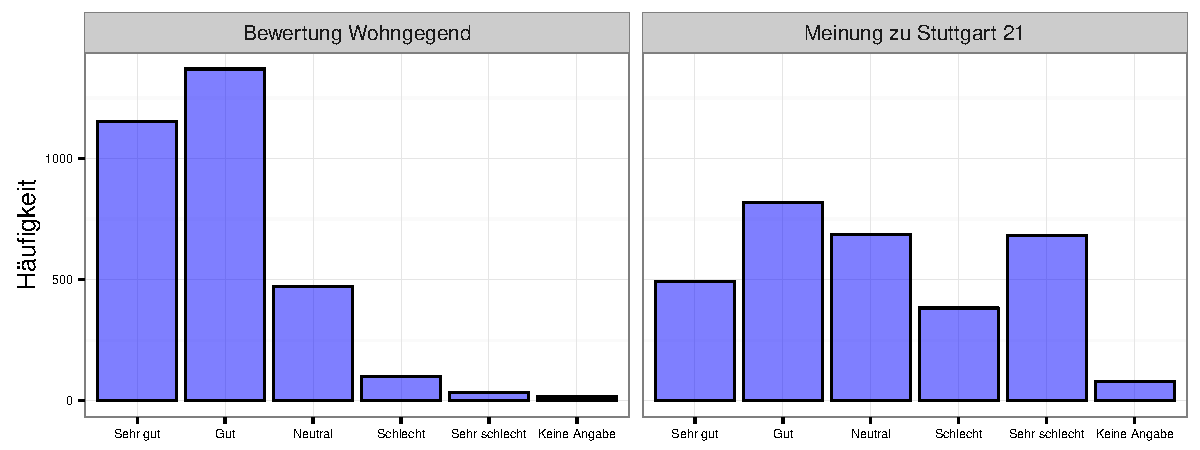
\includegraphics[scale=0.8]{Pictures/BarResp}
 \caption{Häufigkeit der Kategorienausprägungen der endogene Variablen in der Parameterisierungsstichprobe.}
 \label{endogene}
 \end{center}
\end{figure}

Das amtliche, nach Stadtteilen oder Stadtbezirken aufgelöste Ergebnis der Volksabstimmung zu Stuttgart 21 von 2011 kann 
dem Internetauftritt der Stadt entnommen werden \cite{Amt}. Es bietet sich dadurch eine zusätzliche Möglichkeit zur 
Modellevaluierung an, indem die Modellierungsergebnisse mit den tatsächlichen Ergebnissen verglichen werden. Da bei der 
Abstimmung mit Sicherheit nur die beiden Kategorien (\textit{Zustimmung} und \textit{Ablehnung }) unterschieden werden 
können, wurden die Gruppenausprägungen der Parameterisierungsstichprobe neu zusammengefasst. In den Rohdaten wurden noch 
6 Gruppen unterschieden. Es wurde eine Neugruppierung in drei Gruppenausprägungen vorgenommen (Tabelle \ref{endogene}). Dafür wurden jeweils die 
Gruppen \textit{sehr gut} und \textit{gut} zu \textit{Zustimmung} und \textit{schlecht} und \textit{sehr schlecht} zu 
\textit{Ablehnung} zusammengefasst. Falls nur \textit{Zustimmung} und \textit{Ablehnung} für die Modellierung 
berücksichtigt werden sollen, reduziert sich der Stichprobenumfang auf 2377 Beobachtungen. Dadurch bleibt die 
Möglichkeit erhalten eine multinomial verlteilte abhängige Variable zu modellieren und trotzdem eine Validierung für 
zwei Klassen vorzunehmen. Für die exogen in die Analyse einfließenden Variablen sind detailliertere Informationen zu den 
Häufigkeiten der Ausprägungen im Anhang verfügbar (Abbildung \ref{exogen_parametrisierungsdatensatz}). 
\textcolor{red}{bei der abb. Einkommen müsste es $<900$ statt 900 sein}\\

Da in dieser Arbeit ein Schwerpunkt auf der Analyse unterschiedlicher räumlicher Effekte liegt, vergleicht dieser Abschnitt alle drei räumlichen Effekte in Bezug zu den beiden endogenen Variablen. Abbildung \ref{XYStuttgart3} zeigt die absolute Häufigkeit der Beobachtungen der Meinung zu Stuttgart 21 in kontinuierlicher räumlicher Lage. Zur besseren Übersicht wurden nicht alle Beobachtungen geplottet, sondern Beobachtungsdichten über bivariate normalverteilte Kerndichteschätzer mit festem Abstand für jede Richtungen ermittelt \cite{ggplot} sowie \cite{MASS}. Um die Hintergrundkarte einbinden zu können wurden die Gauß-Krüger Koordinaten in Dezimalgrad umgerechnet. Da absolute Dichten dargestellt werden, ist die Dichte der Kategorien nicht nur von der Anzahl der Kategorien selbst, sondern auch von der Einwohnerdichte beeinflusst. Des weiteren wird die Dichte von der Ausschöfung, also der Anzahl beantworteter Befragungsbögen beeinflusst. Wegen der hohen Einwohnerdichte im Innenstadtbereich sind dort die Beobachtungsdichten aller 3 Klassen tendenziell höher als in den Randbezirken. Des weiteren ersichtlich ist, dass einige Bereiche, wie das Naturschutzgebiet \textit{Rotwildpark} im Westen oder der \textit{Schurwald} im Osten, aufgrund ihrer geographischen Beschaffenheit oder Landnutzungsform nicht oder relativ dünn besiedelt sind.

\begin{figure}[h]
 \begin{center}
 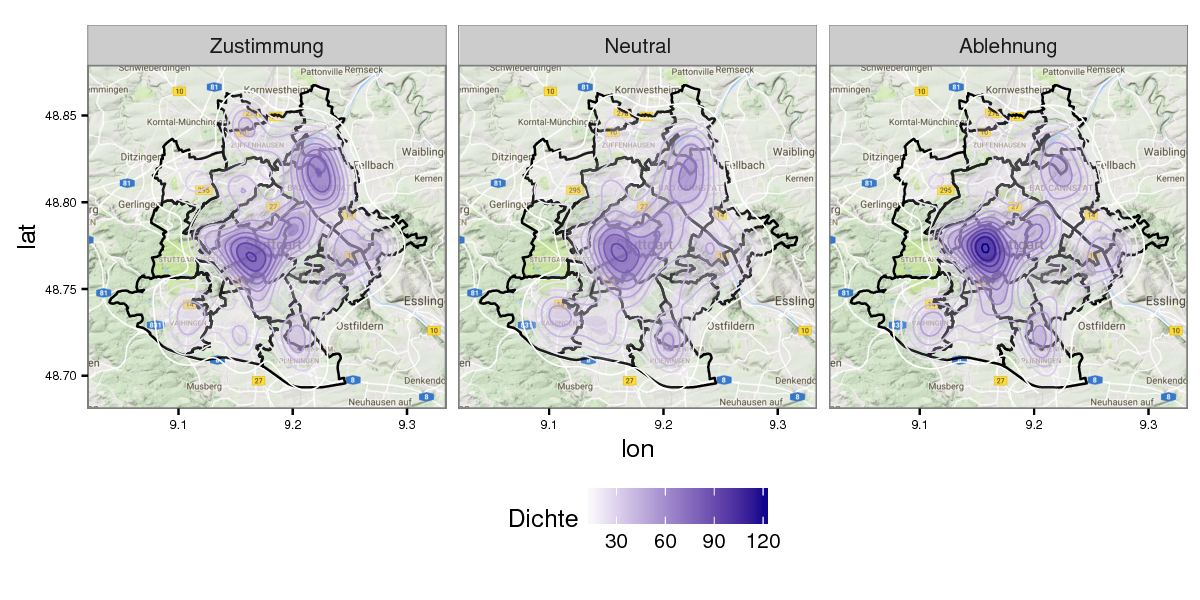
\includegraphics[scale=0.8]{Pictures/XYStuttgart3.png}
 \caption{Kontur Plot der absoluten Anzahl der Gruppenbeobachtungen zur Meinung zu Stuttgart 21 in drei Gruppen. Quelle der Hintergrundgrafik: REF: Google Maps}
 \label{XYStuttgart3}
 \end{center}
\end{figure}

Die \textit{Zustimmung} zeigt offensichtliche räumliche Muster. Im Zentrum und im Nordosten ist sie höher als im Rest 
der Stadt. Der räumliche Trend der \textit{Ablehnung} ist schwächer ausgeprägt. Es zeigt sich jedoch, dass der Bereich 
der Innenstadt, sowie die südlichen Stadtbereiche etwas höhere Dichten bei der \textit{Ablehnung} aufweisen. Die 
Beobachtungen der Kategorie \textit{neutral} sind eher gleichmäßig über die Stadt verteilt.\\
Abbildung \ref{XYWohnG5} zeigt die Dichte der Beobachtungen der fünf Kategorien zur Bewertung der Wohngegend. Hier zeigt sich ein deutlich ausgeprägteres räumliches Muster als bei der Meinung zu Stuttgart 21. Die Beobachtungen der Klasse \textit{sehr gut} häufen sich sehr stark im Innenstadtbereich und im Süden. Die Kategorie \textit{gut} verteilt sich relativ homogen über das gesamte Stadtgebiet mit einer etwas stärkeren Konzentration in der Innenstadt und im Nordosten. Bei der Klasse \textit{neutral} zeigt sich eine stärkere Konzentration auf den Osten und Nordosten der Stadt. Praktisch alle \textit{schlechten} und \textit{sehr schlechten} Bewertungen sind deutlich abgegrenzt im Osten und Nordosten lokalisiert. Hierbei ist zu erwähnen, dass der Anteil der Personen, die ihre Wohngegend mit \textit{schlecht} oder \textit{sehr schlecht} bewertet haben sehr gering ist Abbildung \ref{endogene}.\\

\begin{figure}[h]
 \begin{center}
 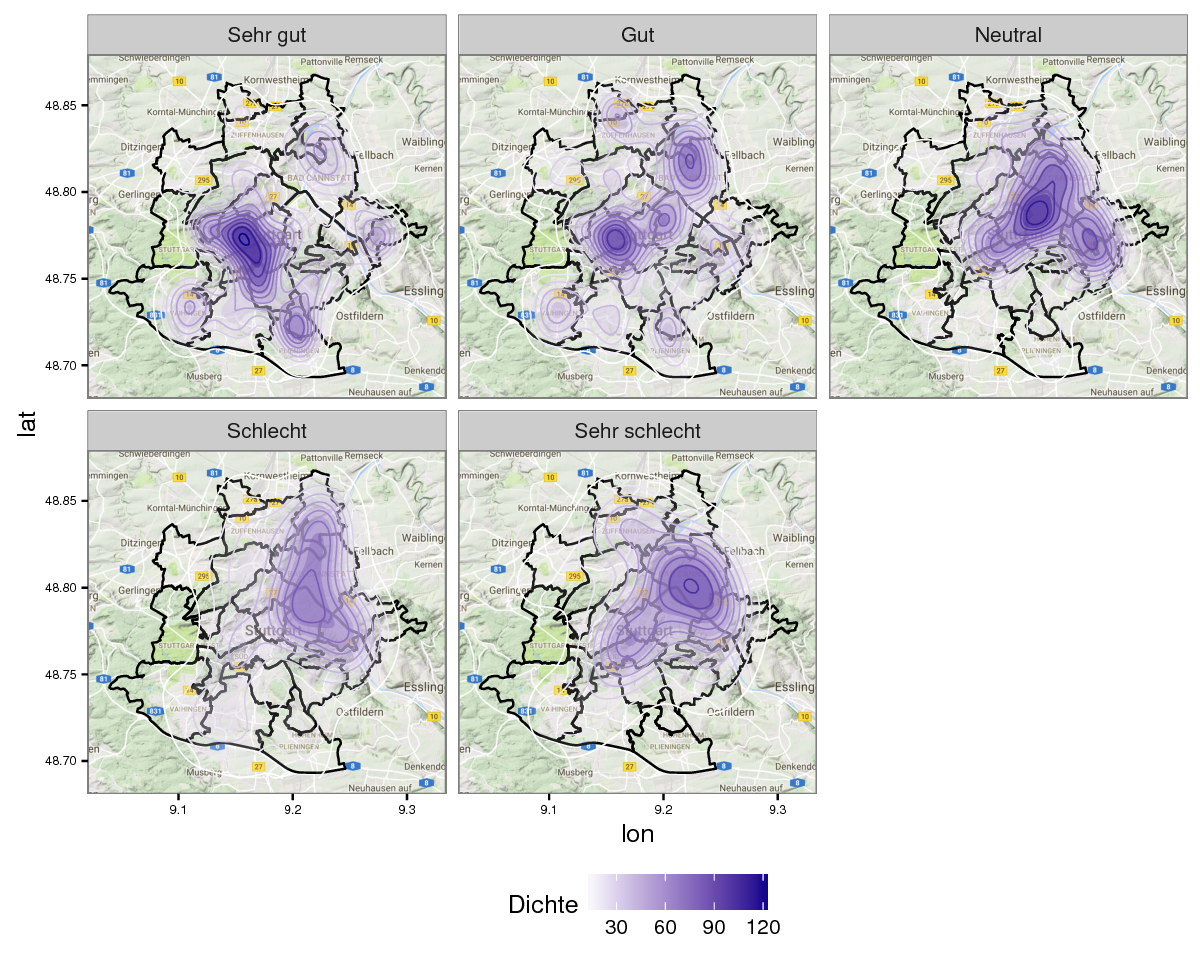
\includegraphics[scale=0.8]{Pictures/XYWohnG5.png}
 \caption{Kontur Plot der absoluten Anzahl der Gruppenbeobachtungen zur Wohnzufriedenheit in fünf Gruppen. Quelle der Hintergrundgrafik: REF: Google Maps}
 \label{XYWohnG5}
 \end{center}
\end{figure}


Im folgenden werden die diskreten räumlichen Informationen auf Stadtbezirksebene beschrieben. Es werden 23 Stadtbezirke 
unterschieden. Im Gegensatz zur stetigen Beobachtungsdichte werden die Beobachtungen nach Regionen aggregiert 
dargestellt. Dies hat den Vorteil, dass eine relative Anteilsdarstellung möglich wird (Abbildung 
\ref{BStuttgart21}). Die absoluten Häufigkeiten sind jedoch nicht dargestellt. Analog zur stetigen Darstellung 
(Abbildung \ref{XYStuttgart3}) ist auch hier zu sehen, dass die Bürger des Nordostens eine positivere Meinung zu 
Stuttgart 21 haben als die Bürger aus dem Süden. Die \textit{neutrale} Klasse hat in allen Bezirken einen geringeren 
Anteil und es ist kein räumliches Muster erkennbar. Die entsprechenden Anteilsgrafiken mit fünf Klassen für die 
Bewertung der Wohngegend sind im Anhang verfügbar (Abbildung \ref{BWohn}). Wie in Abbildung \ref{XYWohnG5} bereits 
angedeutet, zeigen sich negative Wohngebietseinschätzungen vor allem im Nordosten.

\begin{figure}[h]
 \begin{center}
 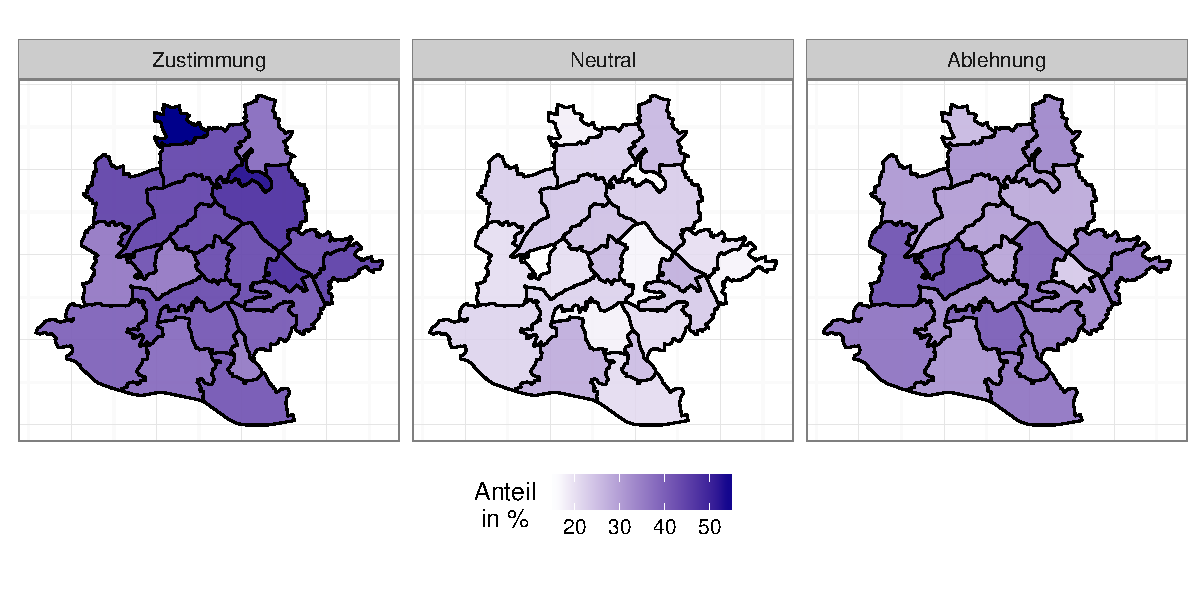
\includegraphics[scale=0.8]{Pictures/BStuttgart3}
 \caption{Anteile zur Meinung zu Stuttgart 21 nach Stadtbezirken.}
 \label{BStuttgart21}
 \end{center}
\end{figure}

Die dritte und letzte untersuchte räumliche Agrregationsebene ist die Stadtteilebene. Abbildung \ref{SStuttgart21} 
zeigt die räumliche Verteilung von \textit{Zustimmung}, \textit{Ablehnung} und \textit{neutraler} Haltung. Wie aus 
Tabelle \ref{Datensatz} hervorgeht, ist die Stadtteilebene deutlich feiner Aufgelöst als die Bezirksebene. Dies führt in 
der Abbildung dazu, dass einige Stadtteile mit geringer Gesamteinwohneranzahl in einer oder mehreren Klassen keine 
Beobachtungen zeigen. Es gibt im Umkehrschluss auch Stadtteile, in denen eine Klasse zu 100 \% vertreten ist. 
Außerdem gibt es in dieser Aggregationsebene sogar Stadtteile ohne jede Beobachtung, wie z. B. das Benzviertel im 
Innenstadtbereich oder die bereits angesprochenen Lagen im Westen.

\begin{figure}[h]
 \begin{center}
 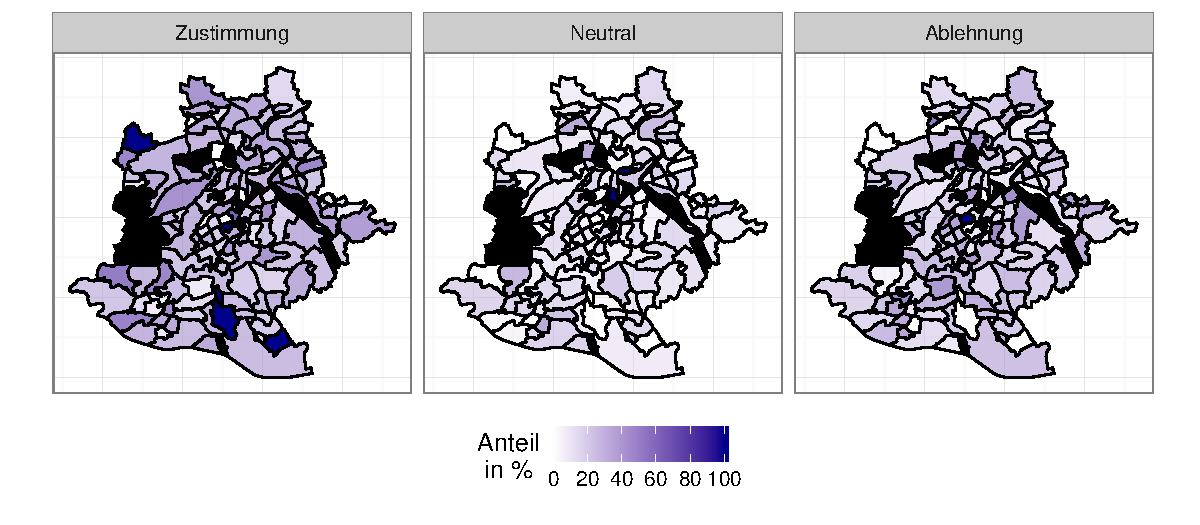
\includegraphics[scale=0.8]{Pictures/SStuttgart3}
 \caption{Anteile der Meinung zu Stuttgart 21 nach Stadtteilen.}
 \label{SStuttgart21}
 \end{center}
\end{figure}

Diese Stadtteile werden in den Diagrammen schwarz dargestellt. Wegen der feineren Auflösung ergibt sich ein 
mosaikartiges, visuell schwerer interpretierbares Bild. In keiner der drei Klassen lässt sich eine klare Struktur oder 
ein räumliches Muster erkennen. Die Anteile auf Stadtteileebene zu der Bewertung der Wohngegend sind im Anhang 
verfügbar \ref{SWohn}. Hier zeigt sich ein ähnlich schwer differenzierbares Muster wie bei der Meinung zu Stuttgart 21. 
Wegen der deutlichen Unterschiede in den Anteilen der fünf Gruppen sind die Farbskalen nicht einheitlich, sondern 
unterscheiden sich in den Diagrammen.\\

\subsubsection{Melderegister}
Die erste Datei an der die Modelle Anwendung finden sollen ist eine personenbezogene Auswertung aus dem Melderegister 
Stuttgarts vom 31.01.2011. Der Auszug umfasst alle volljährigen Einwohner Stuttgarts außer Bewohner von Anstalten und 
Pflegeheimen. Mit einem Stichprobenumfang von 470.190 Bürgern liegt der Melderegisterauszug also sehr nah an 
der Grundgesamtheit von 573.104 Bürgern, die 2011 mit Hauptwohnsitz in Stuttgart gemeldet waren \textcolor{red}{(REF 
Stat. Bundessamt)}. Insgesamt wurden 8 sozioökonomische Variablen erhoben. Bei allen Datensätzen liegt der Wohnsitz als 
kontinuierliche Gauss-Krüger Geokoordinate vor. Um eine kleinräumige Extrapolation mit diskreten räumlichen 
Informationen vornehmen zu können, wurden die Stadtteil- und Stadtbezirksinformationen an die Datensätze des 
Melderegisters angehängt. Hierzu wurden die Stadtteil- und Stadtbezirkspolygone, welche uns von der Stadt Stuttgart für 
die Analyse zur Verfügung gestellt wurden, über eine räumliche Abfrage mit den Melderegisterdatensätzen verknüpft. Die 
geographische Verknüpfung wurde mit dem freien Geoinformationssystem QGIS \textcolor{red}{(REF QGIS)} durchgeführt. Die 
Projektdatei mit der Geoabfrage (\textit{Geographische\_Abfrage.QGS}) sowie die Shapefiledateien 
(\textit{Stadtteile\_netto.SHP}) liegen dieser Arbeit digital bei. Wie in den Tabellen \ref{Datensatz} und 
\ref{Var_Buergerumfrage} ersichtlich, eignen sich nicht alle Variablen zur Extrapolation, da nicht alle Variablen in 
jeder Umfrage erhoben wurden. Es ergibt sich ein Überschneidungsbereich der fünf sozioökonomischen Variablen 
\textit{Altersklasse Befragter}, \textit{Geschlecht}, \textit{Nationalität}, \textit{Familienstand} und 
\textit{Personenzahl im Haushalt}. \textcolor{red}{IN TAB 2 BRAUCHEN WIR DIE SPALTE MODLLEIRUNG EIGENTLICH NICHT MEHR 
ODER? ICH HABE DIE VARIABLEN Z.T. UMBEBENANNT, DAMIT SIE GLEICH HEIßen WIE IN TAB 1. AUßERDEM SIND JA NACH DEM 
UMKODIEREN BEI DER ALTERSKLASSE NUR NOCH  6 AUSPR. ICH WÜRDE DAS IN DER TAB. 2 ANPASSEN WAS MEINST DU?}

\begin{table}[h]
\centering
\caption{Sozioökonomische und geographische Variablen des Melderegisters und deren Anzahl der Ausprägungen.}
\label{Var_Buergerumfrage}
\adjustbox{max height=\dimexpr\textheight-5.5cm\relax,
           max width=\textwidth}{
\begin{tabular}{l|c|c}
\multicolumn{3}{l}{Anzahl Beobachtungen: 470.190}     \\ 
\hline \hline
\textbf{Variable} & \textbf{Modellierung} & \textbf{Anzahl Ausprägungen}  \\ \hline
\multicolumn{1}{l|}{Altersklasse Befragter} &  Nicht Parametrisch & 14 \\ \hline
\multicolumn{1}{l|}{Geschlecht} &  Parametrisch  & 2 \\ \hline
\multicolumn{1}{l|}{Nationalität} & Parametrisch  & 2 \\ \hline
\multicolumn{1}{l|}{Familienstand} & Parametrisch & 4 \\ \hline
\multicolumn{1}{l|}{Personenzahl im Haushalt} &  Nicht Parametrisch  & 5 \\ \hline
\multicolumn{1}{l|}{Wohndauer} & Nicht Parametrisch  & 3 \\ \hline
\multicolumn{1}{l|}{ALG II Quote} & Nicht Parametrisch  & 9 \\ \hline
\multicolumn{1}{l|}{Ein/Zweifamilienhäuser}& Nicht Parametrisch & 8 \\ \hline 
\multicolumn{1}{l|}{Gauß-Krüger} & Tensorprodukt-Splines & \\ \hline \hline
\end{tabular}

}
\end{table}

\subsubsection{Zensus}
Im Rahmen der bundesweiten Volkszählung von 2011 wurde in Stuttgart eine Gebäude- und Wohnungszählung durchgeführt. Diese Datei umfasst 380.238 Bürger Datensätze (Tabelle \ref{Var_Zensus}). Da bei der Zählung auch für die Fragestellung dieser Arbeit relevante sozioökonomische Variablen 
erhoben wurden, eignet sich diese Umfrage ebenfalls zur kleinräumige Extrapolation. Die diskreten geographischen 
Angaben wurden analog zum Vorgehen beim Melderegister per geographischer Abfrage ergänzt. Für die kleinräumige Extrapolation kommen 
die gleichen sozioökonomischen Variablen wie beim Melderegister in Frage. 
\textcolor{red}{Wie in Tab. 2.: Habe die Namen angepasst. Anzahl Personenzahl und Alter umkodiert, also auch in Tabelle 
ändern? Wir könnten sogar überlegen, die nicht verwendeten Variablen zu löschen. Wir gehen ja im Text nicht mehr auf 
diese ein (gilt auch für Tab 2)}

\begin{table}[h]
\centering
\caption{Erhobene sozioökonomische und geographische Variablen der Gebäude- und Wohnungszählung im Rahmen des Zensus und deren Anzahl der Ausprägungen.}
\label{Var_Zensus}
\adjustbox{max height=\dimexpr\textheight-5.5cm\relax,
           max width=\textwidth}{
\begin{tabular}{l|c|c}
\multicolumn{3}{l}{Anzahl Beobachtungen: 380.238}     \\ 
\hline \hline
\textbf{Variable} & \textbf{Modellierung} & \textbf{Mögliche Ausprägungen}  \\ \hline
\multicolumn{1}{l|}{Altersklasse Befragter} &  Nicht Parametrisch & 9 \\ \hline
\multicolumn{1}{l|}{Geschlecht} & Parametrisch  & 2 \\ \hline
\multicolumn{1}{l|}{Nationalität} & Parametrisch  & 2 \\ \hline
\multicolumn{1}{l|}{Familienstand} & Parametrisch & 4 \\ \hline
\multicolumn{1}{l|}{Personenzahl im Hasuhalt} &  Nicht Parametrisch  & 6 \\ \hline
\multicolumn{1}{l|}{Wohnfläche} & Nicht Parametrisch & 24 \\ \hline
\multicolumn{1}{l|}{Stellung Beruf} & Parametrisch  & 9 \\ \hline
\multicolumn{1}{l|}{Beamter}& Parametrisch & 2 \\ \hline 
\multicolumn{1}{l|}{Gebäudetyp}& Parametrisch & 10 \\ \hline
\multicolumn{1}{l|}{Gebäudenutzung}& Parametrisch & 2 \\ \hline
\multicolumn{1}{l|}{Gauß-Krüger} & Tensorprodukt-Splines & \\ \hline \hline
\end{tabular}

}
\end{table}


\subsection{Statistische Methoden}

\subsubsection{Modell}
Bei allen endogenen Variablen handelt es sich um kategorielle Variablen, von denen die Ausprägungswahrscheinlichkeiten modelliert werden sollen. Da Ausprägungswahrscheinlichkeiten für diese kategoriellen Responses nur im Wertebereich zwischen 0 und 1 sinnvoll interpretierbar sind und keine der Response-Variablen Normalverteilung aufweist, sind einfache Regressionsmodelle ohne Transformationsfunktion ungeeignet. Für die Fragestellung dieser Arbeit kommen nur Regressionsmodelle in Frage, die eine Modellierung von Wahrscheinlichkeiten im genannten Wertebereich sicherstellen. Lineare generalisierte Modelle ermöglichen die Transformation des linearen Prädiktors 
$$\eta_{i} =\mathbf{x'}_i \boldsymbol{\beta}$$ 
durch eine Response-Funktion $h$, wobei die Wahl von $h$ von der Fragestellung und der Skalierung der Response-Variable abhängt. $h$ kann jede monoton ansteigende Funktion sein. Zur Sicherstellung des gewünschten Wertebereichs zwischen 0 und 1 wird der lineare Prädiktor bei kategoriellen Regressionen häufig über eine Logit Response-Funktion transformiert. Bei einer binären Response ergibt sich nach \cite[p. 270 f.]{fahrmeir2013regression} folgende Transformation des linearen Prädiktors \textcolor{red}{weißt du, wie man die Formel nummeriert?}
$$h(\eta)=\frac{exp(\eta)}{1+exp(\eta)}$$
Nach einer Logit-Transformation folgen die Daten häufig einer Binomialverteilung. Ein weiterer Vorteil von GLM ist, dass diese spezifischen Verteilungsannahmen berücksichtigt werden können. Bei ordinalskalierter Response kann die Reihenfolge der Ausprägung im generalisierten Modell explizit berücksichtigt werden \cite[p.334 ff.]{fahrmeir2013regression}. Im kumulativen Modell wird angenommen, dass für jeden Datensatz eine kontinuierliche (unbekannte) latente Variable $u_i$ existiert, deren Ausprägung die Kategoriezugehörigkeit bestimmt. Unter der Annahme, dass diese latente Variable über den linearen Prädiktor
$$u_i=-\mathbf{x'}_i \boldsymbol{\tilde{\beta}}+\varepsilon$$
vorhergesagt werden kann, existieren für die latenten Variablen geordnete Schwellenwerte $\theta_{r}$. Damit die Schwellenwerte identifizierbar werden, hat der lineare selbst keinen Intercept. Eine Beobachtung zeigt die Ausprägung $r$, wenn ihre latente Variable zwischen $\theta_{r-1}$ und $\theta_r$ liegt. Über die kumulative Verteilungsfunktion $F$ des Fehlers $\varepsilon_i$ um die latente Variable $u_i$ kann die Wahrscheinlichkeit jeder Ausprägung für jede Beobachtung als 
$$P(y_i=r)=F(\theta_r+\mathbf{x'}_i \boldsymbol{\tilde{\beta}})-F(\theta_{r-1}+\mathbf{x'}_i \boldsymbol{\tilde{\beta}})$$
berechnet werden. Wenn das in der Literatur vorgeschlagene kumulative Logit Modell gewählt wird \cite[p. 334]{fahrmeir2013regression}, berechnet sich die kumulative Wahrscheinlichkeit einer Beobachtung $y_i$ kleiner oder gleich der geordneten Ausprägung $r$ zu sein als
$$P(y_i\leq r)=\frac{exp(\theta_r+\mathbf{x'}_i \boldsymbol{\tilde{\beta}})}{exp(1+exp(\theta_r+\mathbf{x'}_i \boldsymbol{\tilde{\beta}}))}$$\\

Die exogenen Variablen, mit denen das Modell für die räumliche Extrapolation parametrisiert werden soll, sind sehr heterogen. Es kommen sowohl nominal als auch kardinalskalierte sozioökonomischen Variablen in Frage (Abbildung \ref{endogene}, Tabelle \ref{Datensatz}). Während ein linearer Prädiktor zur Beschreibung des Zusammenhangs zwischen ordinalskalierte Variablen und einer kategoriellen Response-Variable ausreichend ist, zeigen kardinal skalierte Variablen oft einen nichtlinearen Zusammenhang \cite[p. 9]{fahrmeir2009regression}. Die in generalisierten linearen Modellen vorausgesetzte lineare Abhängigkeit zwischen allen transformierten Kovariablen und der Response-Variable $\eta$ ist demnach für die Daten dieser Arbeit zu unflexibel. Aufgrund dieser Ausgangslage haben flexiblere Modelle in dieser Arbeit also voraussichtlich Vorteile gegenüber reinen linearen Modellen. Durch generalisierte additive Modelle (GAM) können lineare und nichtlineare Effekte sehr flexibel in einem Modell verbinden werden. Im Unterschied zu generalisierten linearen Modellen sind die einzelnen Terme des Prädiktors nicht auf lineare Funktionen beschränkt, sondern können auch durch semiparametrische Splines nichtlinear modelliert werden. Zurt Modellierung der nichtlinrearen, alos der nichtparametrischen Terme des Prädiktors, wurden penarisierte Basissplines verwendet \cite{eilers1996}. Diese haben den Vorteil, dass 

Analog zu den generalisierten linearen Modellen wird der Prädiktor beim GAM ebenfalls über die Response Logit Response-Funktion transformiert. Im Falle einer binären Response wird die Ausprägungswahrscheinlichkeit über eine Logit Response-Funktion
Je nachdem, ob die Ausprägungswahrscheinlichkeiten für eine Binäre oder geordnet kategorielle Response modelliert werden


ocat, gam \cite{wood2016}


Kurze Erläuterung GAM und logit,... Zusammengesetzt aus parametrischen Effekten und Splines. Pseudobeobachtungen. Wahl 
des Glättungsparameters  (Wood 2000).

\subsubsection{Modellwahl}
Basierend auf den vorhergegangenen Analysen zum Beamten- und Eigenheimanteils in Stuttgart, die uns zur Verfügung standen wurde eine Funktion zur schrittweisen AIC \cite{Akaike1981} Berechnung programmiert, die zur Identifikation der 
geeignetsten Kovariablenkombination dient (siehe digitaler Anhang \textit{stepAIC.R}). In der Funktion werden mithilfe der \texttt{gam()} Funktion des \texttt{mgcv} 
Paketes \cite{Wood2011} generaliserte additive Modelle mit unterschiedlichen Kovariablen erstellt und deren AIC 
berechnet. Vor dem Aufruf der Funktion müssen die abhängige Variable, die Verteilungsannahme des Regressionsmodelles, 
die Gewichtungen der Einzelbeobachtungen und unveränderliche Kovariablen definiert werden. Außerdem muss eingeschätzt 
werden, welche der veränderlichen Kovariablen parametrisch oder semiparametrisch als Spline in das Modell eingehen. Es 
wird zunächst der AIC des einfachsten, nur aus den fest vorgegebenen Kovariablen bestehenden Modells berechnet. In 
Iteration eins werden alle veränderlichen Kovariablen einzeln nacheinander in die Modellformel aufgenommen und es wird 
jeweils ein GAM erstellt sowie dessen AIC berechnet. Die Kovariablen gehen entsprechend der vorigen Eingabe parametrisch 
oder semiparametrisch ein. Falls die Hinzunahme mindestens einer Kovariable in Iteration eins zu einer Reduktion des AIC 
führt, wird diejenige Kovariable, welche zu dem Modell mit dem kleinsten AIC führt zur Modellformel hinzugefügt. Falls 
das Modell nur mit den festen Modellbestandteilen bereits den geringsten AIC zeigt ist die Modellwahl folglich in 
Iteration eins bereits beendet.\\ Andernfalls setzt sich das Ausgangsmodell für Iteration zwei aus den festen 
Kovariablen und einer weiteren Kovariable zusammen. In Iteration zwei werden wie zuvor alle verbleibenden Kovariablen 
zunächst nacheinander zur aktuellen Modellformel hinzugefügt. Wenn die Kovariable mit dem geringsten AIC gefunden ist 
(falls diese existiert und das Modell aus Iteration eins nicht bereits das geeignetste ist), werden alle veränderbaren 
Kovariablen in Iteration zwei nochmals nacheinander eliminiert. Das Modell mit dem geringsten AIC bildet das 
Ausgangsmodell der nächsten Iteration. Dies wird wiederholt bis in einer Iteration kein Modell mit einem geringeren AIC 
als in der vorigen Iteration parametrisiert werden kann. Um die Laufzeit der Funktion zu begrenzen, wurde auf die 
Analyse von Wechselwirkungen zwischen den Kovariablen verzichtet. Wechselwirkungen können jedoch als unveränderliche 
Modellbestandteile eingehen.

\subsubsection{Konfidenzintervalle}
Die Intervalle zu den Punktschätzungen liefern zusätzliche wichtige Informationen, da die Punktschätzungen alleine keine Angaben zur Unsicherheit beinhalten. Das Konfidenzintervall gibt an, mit welcher Wahrscheinlichkeit die unbekannte wahre Punktschätzung von einer Konfidenzregion überdeckt wird. Mit dem Vertrauensintervall erhält man die Relation der Unsicherheit zur Punktschätzung und somit ein weiteres Modellgütemerkmal \cite[p. 471]{fahrmeir2013regression}. Des weiteren wurden die Intervalle genutzt um Überdeckungswahrscheinlichkeiten des Volksabstimmungsergebnisses \cite{Amt} zu berechnen. Grundsätzlich gibt es die Möglichkeiten die Intervalle entweder aus Modelleigenschaften abzuleiten oder Bootstrap-Intervalle durch wiederholte zufällige Modellreparametrisierungen und Punktschätzungen zu berechnen. Bei ersterem Vorgehen unterliegen die Intervallberechnungen, je nach gewählter Berechnungsmethode, asymptotischen Eigenschaften oder Verteilungsannahmen. So wird zur analytischen Berechnung von Score-Konfidenzintervallen \cite[p. 64 ff.]{held2008}, welche den Vorteil haben, dass sie invariant gegenüber eindeutigen Parametertransformationen sind, beispielsweise die Fischer-Information benötigt. Sie sind deshalb oft nur schwer analytisch zu berechnen \cite[p. 74]{held2008}. Andere Intervalle, wie bespielsweise das Wald-Konfidenzintervall, sind obligatorisch symmetrisch \cite[p. 60]{held2008} und werden der wahren Datenverteilung daher oft nicht gerecht. Bei beiden Intervallen hängt die tatsächliche Überdeckungswahrscheinlichkeit dea unbekannten wahren Parametera bei binärer Response Variable zudem von der Parameterausprägung sowie der Beobachtungsanzahl der Modellstichprobe ab und entspricht deshalb in ungünstigen Kombinationen nicht der nominellen, also der gewünschten Überdeckungswahrscheinlichkeit \cite{Int}. 
\\Bootstrap Konfidenzintervalle hingegen können für jede Form der statistischen Inferenz berechnet werden \cite{diciccio1996}. Da in dieser Arbeit Modelle mit unterschiedlichen Verteilungsannahmen und unterschiedlichen räumlichen Effekten vergleichen werden, bieteten es sich an auf die verteilungsunabhängigen Bootstrap-Intervallschätzungen zurückzugreifen. Von Interesse sind weniger die Intervalle um die Modellparameter als vielmehr die Intervalle um die Punktschätzungen, also die einzelnen Hochrechnungen. Dementsprechend wurden Bootstrap-Konfidenzintervalle für jede einzelne Punktschätzung berechnet. Zur Berechnung der Intervalle wurde jedes Modell 1.000 mal mit einer Zufallsstichprobe (\textit{Ziehen-mit-Zurücklegen}) aus der Parameterisierungsstichprobe reprametrisiert. Um den Einfluss des Stichprobenumfangs zu eliminieren, enthielt jede Stichprobe die tatsächliche Anzahl der Beobachtungen. Mit jedem neuparametrisierten Modell wurde eine kleinräumige Extrapolation durchgeführt. Die Hochrechnungsergebnisse wurden genutzt um die arithmetischen Mittel, die Mediane sowie untere und obere 95 \% Perzentile der Punktschätzungen zu berechnen.

\subsubsection{Kreuzvalidierung}
Für die Modellerstellung der additiven Modelle lag eine Stichprobe von 3.143 Beobachtungen vor. Informationen zur Grundgesamtheit dieser Stichprobe lagen nicht vor. Die Qualität der parametrisierten Modelle ließ sich folglich nicht anhand einer Grundgesamtheit validieren, sondern musste an der Stichprobe selbst eingeschätzt werden. Die erstellten Modelle wurden an anderen Dat3en als den Parametrisierungsdaten angewendet. Aus diesem Grunde ist war vor allem die Modellqualität außerhalb der Parametrisierungsdaten interessant. Aus diesem Grunde wurde eine \textit{Leave-One-Out} Kreuzvalidierung durchgeführt \cite[p. 149]{fahrmeir2013regression}, in welcher jeweils eine Beobachtung zufällig entfernt wurde. Mit den verbliebenen Datensätzen wurde das additive Modell, welches sich zuvor im schrittweisen AIC Vergleich als am vorteilhaftesten herausgestellt hat, neu parametrisiert und die entfernte Beobachtung mit diesem Modell vorhergesagt. Dies wurde so lange wiederholt bis jeder Datensatz einmal entfernt (und geschätzt) wurde. Mit diesen Daten ließ sich eine Statistik zur Reklassifikation der Beobachtungen außerhalb der Stichprobe erstellen.

\subsubsection{Validierung}
Ziel der Validierung ist es, die prognostizierten Anteile aus dem gewählten Modell mit den wahren Anteilen aus der 
Volksabstimmung \cite{Amt} zu vergleichen, um eine Aussage über die Qualität der geschätzten Prognosemodelle geben zu 
können. Die Validierung erfolgt auf Stadtteil- und Bezirksebene, sowie für das Gesamtergebnis der Stadt Stuttgart. Dazu 
werden insbesondere zwei statistische Gütemaße verwendet.\\
Bei der Wahl des Schätzers geht es zum einen darum, einen möglichst erwartungstreuen als auch effizienten Schätzer zu 
finden. Als geeignetes Gütemaß hat sich die mittlere quadratische Abweichung erwiesen, da sie sowohl die Varianz, als 
auch die quadrierte Verzerrung berücksichtigt. Zudem hat ein konsistenter Schätzer die Eigenschaft, dass die mittlere 
quadratische Abweichung bei unendlich groß werdender Stichprobe gen Null konvergiert \cite[p. 201]{HOG}. Ein weiteres 
Kriterium ist die Überdeckungswahrscheinlichkeit. Sie gibt an, mit welcher Wahrscheinlichkeit das geschätzte 
Konfidenzintervall den wahren Wert enthält. Erwartet wird hier, dass die Überdeckungswahrscheinlichkeit dem 
Konfidenzniveau entspricht. Mögliche größere Abweichungen können durch die Approximation einer diskreten Verteilung 
durch eine stetige Verteilung resultieren, was z.B. oft bei der Approximation der Binomial- durch die Normalverteilung 
vorkommt \cite[p. 102]{Int}.

\section{Ergebnisse}


\subsection{Modell}

\subsection{Modellwahl}

Die Modellwahl mit Hilfe der Funktion \texttt{stepAIC} hat eine Zusammensetzung von Kovariablen geliefert, welche das Modell mit dem besten Fit und der geringsten Komplexität liefert. Da der räumliche Effekt stets als fester Bestandteil aufgenommen wurde, listest Tabelle \ref{stepAIC} zu jedem Modell das AIC für ein vollständiges Geoadditives Modell, einem Modell nur mit räumlichem Effekt und ein Modell bestehend aus allen Kovariablen außer dem räumlichem Effekt auf. Dadurch lässt sich die relative Informationsqualität des jeweiligen räumlichen Effekts untersuchen. \\
Für die Meinung zu Stuttgart 21 im drei Klassen Fall lässt sich erkennen, dass das Geoadditive Modell mit den Gauss-Krüger Informationen und den Stadtteil Informationen die höchste relative Qualität aufweist. Bei dem Modell mit Bezirken als räumlichem Effekt scheint dieser die Qualität des Modells in Abhängigkeit von der Komplexität nicht zu verbessern. Insgesamt deutet das AIC für den drei Klassen Fall auf das Geoadditive Modell mit den Gauss-Krüger Informationen als qualitativ höchstes Modell hin. Beim zwei Klassen Fall schneidet das Geoadditive Modell in jedem Fall am besten ab, wobei hier das Modell mit Stadtteilen als räumlichem Effekt die höchste Qualität laut des AIC aufweist.

\begin{table}[h]
\centering
\caption{Vergleich der step AIC Ergebnisse zwischen den Modellen}
\label{stepAIC}
\begin{tabular}{llccc}
\hline \hline
\multicolumn{5}{c}{Meinung zu Stuttgart 21}                                                                                                                                            \\ \hline
                          & \multicolumn{1}{l|}{}             & \multicolumn{1}{c|}{\multirow{2}{*}{Geoadditives Modell}} & \multicolumn{1}{c|}{Modell ohne}       & Modell nur mit    \\
                          & \multicolumn{1}{l|}{}             & \multicolumn{1}{c|}{}                                     & \multicolumn{1}{c|}{räumlichem Effekt} & räumlichem Effekt \\ \hline
\multirow{3}{*}{Drei Kl.} & \multicolumn{1}{l|}{Gauss-Krüger} & \multicolumn{1}{c|}{6379,345}                             & \multicolumn{1}{c|}{6382,654}          & 6456,846          \\
                          & \multicolumn{1}{l|}{Bezirke}      & \multicolumn{1}{c|}{6455,284}                             & \multicolumn{1}{c|}{6383}              & 6455,284          \\
                          & \multicolumn{1}{l|}{Stadtteile}   & \multicolumn{1}{c|}{6428,6}                               & \multicolumn{1}{c|}{6509,871}          & 6510,838          \\ \hline
\multirow{3}{*}{Zwei Kl.} & \multicolumn{1}{l|}{Gauss-Krüger} & \multicolumn{1}{c|}{3114,143}                             & \multicolumn{1}{c|}{3116.13}           & 3268,483          \\
                          & \multicolumn{1}{l|}{Bezirke}      & \multicolumn{1}{c|}{3115,858}                             & \multicolumn{1}{c|}{3116.13}           & 3271,325          \\
                          & \multicolumn{1}{l|}{Stadtteile}   & \multicolumn{1}{c|}{3079,12}                              & \multicolumn{1}{c|}{3117.902}          & 3163,597          \\ \hline
\multicolumn{5}{c}{Bewertung der Wohngegend}                                                                                                                                           \\ \hline
                          & \multicolumn{1}{l|}{}             & \multicolumn{1}{c|}{\multirow{2}{*}{Geoadditives Modell}} & \multicolumn{1}{c|}{Modell ohne}       & Modell nur mit    \\
                          & \multicolumn{1}{l|}{}             & \multicolumn{1}{c|}{}                                     & \multicolumn{1}{c|}{räumlichem Effekt} & räumlichem Effekt \\ \hline
                          & \multicolumn{1}{l|}{Gauss-Krüger} & \multicolumn{1}{c|}{7051,606}                             & \multicolumn{1}{c|}{7318,815}          & 7062,108          \\
                          & \multicolumn{1}{l|}{Bezirke}      & \multicolumn{1}{c|}{7175,601}                             & \multicolumn{1}{c|}{7318,815}          & 7197,003          \\
                          & \multicolumn{1}{l|}{Stadtteile}   & \multicolumn{1}{c|}{8252,374}                             & \multicolumn{1}{c|}{8567,358}          & 8750,801          \\ \hline \hline
\end{tabular}
\end{table}

Für die Bewertung der Wohngegend als endogene Variable zeigt sich noch ein deutlicherer Unterschied zwischen Schätzungen mit räumlichem Effekt und ohne räumlichem Effekt. Modelle mit räumlichem Effekt zeigen einen deutlich niedrigeren AIC, so ist der Unterschied bei den Gauss-Krüger und Bezirksinformationen zwischen dem Geoaddtitven Modell und dem Modell nur mit räumlichem Effekt sehr viel geringer ist als zwischen Geoadditivem Modell und Modell ohne räumlichem Effekt. Dies weißt darauf hin, dass der räumliche Effekt einen hohen Erklärungsgehalt für die Ausprägung der abhängigen Variable liefert. Die gegenteilige Situation findet man bei der Meinung zu Stuttgart 21 vor. Insgesamt signalisiert das AIC die höchste Qualität für das Geoadditive Modell mit Gauss-Krüger Informationen bei der Bewertung der Wohngegend.

\subsection{Reklassifizierung}

Die Ergebnisse der Reklassifizierung zur Meinung zu Stuttgart 21 (Tabelle \ref{evalS21}) zeigen, dass die Erfolgsquote im drei Klassenmodell zwischen 44\% und 50\% liegt und im zwei Klassenmodell zwischen 55\% und 62\% liegt. Zum Vergleich mit einem reinen Zufallsmodell, dass im drei Klassenmodell eine Erfolgswahrscheinlichkeit von 1/3 und im zwei Klassenmodell von 1/2 hat, weißen die geschätzten Modelle eine höhere Erfolgsquote auf. Auch bei einem Vergleich mit Tabelle \ref{endogene} zeigt sich, dass die geschätzten Modelle besser abschneiden, als ein triviales Wählen der immer gleichen Klasse.

\begin{table}[h]
\centering
\caption{Reklassifizierung der Meinung zu Stuttgart 21}
\label{evalS21}
\begin{tabular}{ll|c|c|c}
\hline \hline
                          &              & \multirow{2}{*}{Geoadditives Modell} & Modell ohne       & Modell nur mit    \\
                          &              &                                      & räumlichem Effekt & räumlichem Effekt \\ \hline
\multirow{3}{*}{Drei Kl.} & Gauss-Krüger & 0,4918                               & 0,4716            & 0,4732            \\
                          & Bezirke      & 0,4726                               & 0,4719            & 0,4726            \\
                          & Stadtteile   & 0,451                                & 0,4685            & 0,4449            \\ \hline
\multirow{3}{*}{Zwei Kl.} & Gauss-Krüger & 0,6193                               & 0,6104            & 0,5524            \\
                          & Bezirke      & 0,6079                               & 0,6104            & 0,5515            \\
                          & Stadtteile   & 0,6282                               & 0,6052            & 0,6099            \\ \hline \hline
\end{tabular}
\end{table}

Des weiteren ist zu sehen, dass das Geoadditive Modell in fast allen Fällen die höchste Erfolgsquote aufweist. Abweichungen bestehen im drei Klassenmodell mit Stadtteilen als räumlichem Effekt und im zwei Klassenmodell mit Bezirken als räumlichem Effekt. Außerdem ist zu beachten, dass im drei Klassenmodell das Modell nur mit räumlichem Effekt besser abschneidet als das Modell ohne räumlichem Effekt, während sich für zwei Klassen diese Situation umgekehrt hat.\\
Für die Reklassifikation der Bewertung der Wohngegend (Tabelle \ref{evalB}) ergibt sich eine Erfolgsquote zwischen 40\% und 50\%. Damit ist auch hier eine deutliche Verbesserung gegenüber reinem Raten oder dauerhaftem wählen einer Klasse gegeben. 

\begin{table}[h]
\centering
\caption{Reklassifizierung der Bewertung der Wohngegend}
\label{evalB}
\begin{tabular}{l|c|c|c}
\hline \hline
             & \multirow{2}{*}{Geoadditives Modell} & Modell ohne       & Modell nur mit    \\
             &                                      & räumlichem Effekt & räumlichem Effekt \\ \hline
Gauss-Krüger & 0,4922                               & 0,4461            & 0,4896            \\
Bezirke      & 0,4701                               & 0,4461            & 0,4621            \\
Stadtteile   & 0,4046                               & 0,4204            & 0,4347            \\ \hline \hline
\end{tabular}
\end{table}

Für die Modelle mit den kontinuierlichen Gauss-Krüger Informationen und den Bezirken als räumlichem Effekt hat das Geoadditive Modell die höchste Erfolgsrate, wohingegen für die Stadtteilinformationen das Modell nur mit räumlichem Effekt die beste Reklassifizierung aufweist. Insgesamt schneidet das Geoadditive Modell für beide endogene Variablen und alle drei möglichen Klassenanzahlen am besten ab. Außer bei dem zwei Klassenmodell zur Meinung zu Stuttgart 21 weisen beim Geoadditivem Modell die Gauss-Krüger Informationen als räumliche Effekte die höchste und die Stadtteile als räumliche Effekte die niedrigste Erfolgsrate auf. Da die Modelle ohne- oder nur mit räumlichem Effekt in der AIC-Untersuchung und Reklassifizierung in den meisten Fällen schlechter Abschnitten, wurden die Ansätze ohne- oder nur mit räumlichem Effekte nicht weiter verfolgt.

\subsection{Kreuzvalidierung}

Die Kreuzvalidierung wurde vorgenommen, um die Vorhersagequalität außerhalb der eigenen Stichprobe der Modelle einzuschätzen. Die Ergebnisse zur Meinung zu Stuttgart 21 (Tabelle \ref{KreuzM}) zeigen eine ähnliche Erfolgsquote wie die innerhalb der Stichprobe vorgenommene Reklassifizierung (Tabelle \ref{evalS21}). Für das drei Klassenmodell liegt der Anteil der erfolgreich Klassifizierten Beobachtungen bei ca. 49\% und im zwei Klassenmodell zwischen 60\% und 63\%. Im drei Klassen Fall kann das Modell mit Stadtteilen als räumlichem Effekt ca. 3,5\%  mehr Beobachtungen richtig zuweisen als in der Reklassifizierung und das Modell mit Bezirken als räumlichem Effekt ca. 2\%, womit es insgesamt auch die höchste Erfolgsrate aufweist. Die Erfolgsquote mit den Gauss-Krüger Informationen ist in etwa gleich geblieben, ähnlich wie die Modelle im zwei Klassen Fall.
 
\begin{table}[h]
\centering
\caption{Kreuzvalidierung der Meinung zu Stuttgart 21 nach einzelnen Klassen}
\label{KreuzM}
\begin{tabular}{lcccccccccc}
\hline \hline
\multicolumn{11}{c}{Drei Klassen}                                                                                                                                                                                                        \\ \hline 
\multicolumn{1}{c}{}                                                     & \multicolumn{1}{c|}{}  & \multicolumn{3}{c|}{Gauss-Krüger}            & \multicolumn{3}{c|}{Bezirke}                 & \multicolumn{3}{c}{Stadtteile}         \\ \cline{3-11} 
                                                                         & \multicolumn{1}{c|}{}  & \multicolumn{9}{c}{Geschätzte Klasse}                                                                                                \\
                                                                         & \multicolumn{1}{c|}{}  & 1       & 2   & \multicolumn{1}{c|}{3}       & 1       & 2   & \multicolumn{1}{c|}{3}       & 1           & 2           & 3          \\ \hline
\multirow{3}{*}{\begin{tabular}[c]{@{}l@{}}Wahre \\ Klasse \end{tabular}} & \multicolumn{1}{c|}{1} & 0,756   & 0   & \multicolumn{1}{c|}{0,244}   & 0,754   & 0   & \multicolumn{1}{c|}{0,246}   & 0,746           & 0           & 0,254        \\
                                                                         & \multicolumn{1}{c|}{2} & 0,673   & 0   & \multicolumn{1}{c|}{0,327}   & 0,670   & 0   & \multicolumn{1}{c|}{0,330}   & 0,663          & 0           & 0,337        \\
                                                                         & \multicolumn{1}{c|}{3} & 0,521   & 0   & \multicolumn{1}{c|}{0,479}   & 0,511   & 0   & \multicolumn{1}{c|}{0,489}   & 0,509      & 0           & 0.491     \\ \hline
\multicolumn{2}{l|}{Klassifikation Modell}                                                        & \multicolumn{3}{c|}{\multirow{2}{*}{0,4905}} & \multicolumn{3}{c|}{\multirow{2}{*}{0,4928}} & \multicolumn{3}{c}{\multirow{2}{*}{0,4893}} \\
\multicolumn{2}{l|}{Insgeasmt}                                                                    & \multicolumn{3}{c|}{}                        & \multicolumn{3}{c|}{}                        & \multicolumn{3}{c}{}                   \\ \hline
\multicolumn{11}{c}{Zwei Klassen}                                                                                                                                                                                                        \\ \hline
                                                                         & \multicolumn{1}{l|}{}  & \multicolumn{3}{c}{Gauss-Krüger}             & \multicolumn{3}{c}{Bezirke}                  & \multicolumn{3}{c}{Stadtteile}         \\ \cline{3-11} 
                                                                         & \multicolumn{1}{l|}{}  & \multicolumn{9}{c}{Geschätzte Klasse}                                                                                                \\
                                                                         & \multicolumn{1}{l|}{}  & 1       & \multicolumn{2}{c|}{2}             & 1       & \multicolumn{2}{c|}{2}             & 1           & \multicolumn{2}{c}{2}    \\ \hline
Wahre                                                                    & \multicolumn{1}{l|}{1} & 0,747   & \multicolumn{2}{c|}{0,253}         & 0,732   & \multicolumn{2}{c|}{0,268}         & 0,748         & \multicolumn{2}{c}{0,252}    \\
Klasse                                                                   & \multicolumn{1}{l|}{2} & 0,538   & \multicolumn{2}{c|}{0,462}         & 0,545   & \multicolumn{2}{c|}{0,455}         & 0,516       & \multicolumn{2}{c}{0,484}    \\ \hline
\multicolumn{2}{l|}{Klassifikation Modell}                                                        & \multicolumn{3}{c|}{\multirow{2}{*}{0,6193}} & \multicolumn{3}{c|}{\multirow{2}{*}{0,6079}} & \multicolumn{3}{c}{\multirow{2}{*}{0,6286}} \\
\multicolumn{2}{l|}{Insgesamt}                                                                    & \multicolumn{3}{c|}{}                        & \multicolumn{3}{c|}{}                        & \multicolumn{3}{c}{}                   \\ \hline \hline
\end{tabular}
\end{table}

Zudem lässt sich anhand von Tabelle \ref{evalS21} die Trefferquote der einzelnen Klassen entnehmen. Die Tabelle zeigt die Anteile der Zuordnung von Beobachtungen der jeweiligen Klasse auf die eigene und jede der anderen Klassen. Die Hauptdiagonale liefert die Anteile der korrekt zugeordneten Beobachtungen. Die Einträge auf den Nebendiagonalen geben damit an, wie viele Beobachtungen einer Klasse relativ zur Gesamtzahl der Beobachtungen in eine falsche Klasse zugeordnet wurden. Markant ist, dass der zweiten Klasse in keinem Modell Beobachtungen zugeordnet wurden, weder falsch noch richtig. Mehrheitlich wurden diese der ersten Kategorie zugewiesen. Zudem ist die erste Klasse am öftesten richtig zugeordnet worden, allerdings wurden ihr auch die meisten falsch klassifizierten Beobachtungen zugeordnet. Dies gilt für alle drei Modelle. Im zwei Klassen Fall wurde das Problem der nicht geschätzten zweiten Klasse durch ihr auslassen umgangen. Allerdings findet sich auch hier ein deutlich häufigeres falsches zuordnen der zweiten Klasse in die erste als anders herum. 

\begin{table}[h]
\centering
\caption{Kreuzvalidierung der Bewertung der Wohngegend nach einzelnen Klassen}
\label{KreuzBew}
\begin{tabular}{lc|ccccccccccccccc}
\hline \hline
\multicolumn{1}{c}{}                                                     &   & \multicolumn{5}{c|}{Gauss-Krüger}              & \multicolumn{5}{c|}{Bezirke}                   & \multicolumn{5}{c}{Stadtteile}              \\ \cline{3-17} 
                                                                         &   & \multicolumn{15}{c}{Geschätzte Klasse}                                                                                                        \\
                                                                         &   & 1     & 2     & 3 & 4 & \multicolumn{1}{c|}{5} & 1     & 2     & 3 & 4 & \multicolumn{1}{c|}{5} & 1       & 2       & 3       & 4   & 5       \\ \hline
\multirow{5}{*}{\begin{tabular}[c]{@{}l@{}}Wahre \\ Klasse\end{tabular}} & 1 & 0,445 & 0,555 & 0 & 0 & \multicolumn{1}{c|}{0} & 0,387 & 0,613 & 0 & 0 & \multicolumn{1}{c|}{0} & 0,495   & 0,478   & 0,019   & 0   & 0,008   \\
                                                                         & 2 & 0,254 & 0,746 & 0 & 0 & \multicolumn{1}{c|}{0} & 0,252 & 0,748 & 0 & 0 & \multicolumn{1}{c|}{0} & 0,300   & 0,671   & 0,023   & 0   & 0,006   \\
                                                                         & 3 & 0,149 & 0,845 & 0 & 0 & \multicolumn{1}{c|}{0} & 0,153 & 0,847 & 0 & 0 & \multicolumn{1}{c|}{0} & 0,142   & 0,771   & 0,079   & 0   & 0,008   \\
                                                                         & 4 & 0,141 & 0,859 & 0 & 0 & \multicolumn{1}{c|}{0} & 0,141 & 0,859 & 0 & 0 & \multicolumn{1}{c|}{0} & 0,099   & 0,474   & 0,349   & 0   & 0,078   \\
                                                                         & 5 & 0,114 & 0,886 & 0 & 0 & \multicolumn{1}{c|}{0} & 0,086 & 0,914 & 0 & 0 & \multicolumn{1}{c|}{0} & 0,031   & 0,275   & 0,556   & 0   & 0,138   \\ \hline
\multicolumn{2}{l|}{Klassifik.}                                              & \multicolumn{5}{c|}{\multirow{3}{*}{0.4918}}   & \multicolumn{5}{c|}{\multirow{3}{*}{0,4704}}   & \multicolumn{5}{c}{\multirow{3}{*}{0,4594}} \\
\multicolumn{2}{l|}{Modell}                                                  & \multicolumn{5}{c|}{}                          & \multicolumn{5}{c|}{}                          & \multicolumn{5}{c}{}                        \\
\multicolumn{2}{l|}{Insgesamt}                                               & \multicolumn{5}{c|}{}                          & \multicolumn{5}{c|}{}                          & \multicolumn{5}{c}{}                        \\ \hline  \hline
\end{tabular}
\end{table}

Tabelle \ref{evalB} ist analog zu Tabelle \ref{evalS21} aufgebaut. Das Ergebnis der Kreuzvalidierung für die Bewertung der Wohngegend ist, dass die Erfolgsquote zwischen ca. 46\% und 49\% liegt. Die Modelle mit Gauss-Krüger Informationen und Bezirken als räumliche Effekte haben vergleichbar wie in der Reklassifizierung abgeschnitten. Das Modell mit den Stadtteilen hingegen weißt eine ca 5\% höhere Genauigkeit auf. Insgesamt jedoch behält das Modell mit den Gauss-Krüger Informationen die höchste Erfolgsrate. Auffällig ist auch hier, dass eine Klasse in keinem Modell Beobachtungen zugewiesen bekommen hat und zwei weitere Klassen in zwei von drei Modellen keine Beobachtungen zugewiesen bekommen haben. Abbildung \ref{endogene} gibt dabei einen Hinweis auf die Ursache dieses Phänomens, denn die Kategorien \textit{sehr gut} und \textit{gut} sind überproportional häufig im Datensatz vertreten im Vergleich zu den Klassen \textit{schlecht} und \textit{sehr schlecht}, weshalb schon durch die relative Häufigkeit die Wahrscheinlichkeit dass eine Beobachtungen in einer der letzten drei Kategorien ist, sehr klein wird. Bei der Bewertung der Wohngegend wurde am häufigsten die zweite Klasse sowohl richtig als auch falsch geschätzt.\\
Durch das relativ hohe Überschätzen einer Klasse bei beiden endogenen Variablen, sowie das totale Unterschätzen einiger Klassen, wird in der weiteren Validierung und Extrapolation auf das Vorhersagen einzelner Beobachtungen verzichtet. Stattdessen wird in einem bestimmten Gebiet über die Wahrscheinlichkeiten der Beobachtungen aggregiert und ein Anteil geschätzt, um auch geringere Wahrscheinlichkeiten für Beobachtungen zu berücksichtigen.

\subsection{Validierung}

Die Ergebnisse der Validierung sind aus Tabelle \ref{vali} ersichtlich. Die Tabelle zeigt die mittlere Quadratische Abweichung und Überdeckungswahrscheinlichkeit der prognostizierten Anteile aus den Modellen, bezogen auf die wahren Anteile aus der Volksabstimmung. Da in dieser Volksabstimmung nur Informationen zu zwei Klassen verfügbar sind, wird erwartet, dass das zwei Klassenmodell die beiden Kategorien signifikant besser prognostiziert.
Tabelle \ref{vali} ist so aufgebaut, dass die linke Spalte angibt um welche Kombination aus Modell, räumlichem Effekt und Datei es sich handelt. Die mittlere Spalte zeigt die mittlere quadratische Abweichung für die beiden Kategorien der Volksabstimmung und die rechte Spalte zeigt die Überdeckungswahrscheinlichkeit ebenfalls für diese Kategorien. Damit gibt die erste Reihe z.B. die statistischen Gütemaße für das zwei Klassenmodell mit Gauss-Krüger Informationen als räumlichem Effekt aggregiert auf Bezirksebene mit dem Melderegister an.

\begin{table}[h]
\centering
\caption{Vergleich der mittleren quadratischen Abweichung (MSE) und der Überdeckungswahrscheinlichkeit bei allen Prognosen aus den geschätzten Modellen und den beiden Extrapolationsdateien für die Meinung zu Stuttgart 21}
\label{vali}
\begin{tabular}{llll|cc|cc}
\hline \hline
                        &                               &                          &   & \multicolumn{2}{c|}{MSE} & \multicolumn{2}{c}{Überdeckungswk.} \\
                        &                               &                          &   & Zustimmung  & Ablehnung  & Zustimmung        & Ablehnung       \\ \hline
\multirow{12}{*}{3 Kl.} & \multirow{4}{*}{Gauss-Krüger} & \multirow{2}{*}{Bez.}    & U & 0,04        & 0,749      & 1                 & 0,043           \\
                        &                               &                          & Z & 0,116       & 0,557      & 0,391             & 0               \\ \cline{3-8} 
                        &                               & \multirow{2}{*}{Sadtt.}  & U & 0,461       & 5,708      & 0,954             & 0,139           \\
                        &                               &                          & Z & 0,813       & 4,415      & 0,553             & 0,02            \\ \cline{2-8} 
                        & \multirow{4}{*}{Bezirke}      & \multirow{2}{*}{Bez.}    & U & 0,041       & 0,756      & 1                 & 0,043           \\
                        &                               &                          & Z & 0,117       & 0,562      & 0,522             & 0               \\ \cline{3-8} 
                        &                               & \multirow{2}{*}{Stadtt.} & U & 0,482       & 5,678      & 0,934             & 0,139           \\
                        &                               &                          & Z & 0,835       & 4,38       & 0,567             & 0,027           \\ \cline{2-8} 
                        & \multirow{4}{*}{Stadtteile}   & \multirow{2}{*}{Bez.}    & U & 0,032      & 0,862     &      1             &   0,043          \\
                        &                               &                          & Z & 0,148       & 0,552      &     0,478         &     0 \\ \cline{3-8} 
                        &                               & \multirow{2}{*}{Stadtt.} & U & 0,646       & 6,367       &   0,947           &   0,225  \\
                        &                               &                          & Z & 1,078        & 4,336       &   0,66           &                0,1 \\ \hline
\multirow{12}{*}{2 Kl.}  & \multirow{4}{*}{Gauss-Krüger} & \multirow{2}{*}{Bez.}   & U & 0,312      & 0,312      &     0,826           &  0,826
 \\
                        &                               &                          & Z & 0,152      & 0,152      &   0,522           &  0,522     \\ \cline{3-8} 
                        &                               & \multirow{2}{*}{Stadtt.} & U & 2,694       & 2,679     &   0,649          &  0,649   \\
                        &                               &                          & Z & 1,581       & 1,569      &  0,46            &   0,46   \\ \cline{2-8} 
                        & \multirow{4}{*}{Bezirke}      & \multirow{2}{*}{Bez.}    & U & 0,312       & 0,312      &  0,826            &   0,826    \\
                        &                               &                          & Z & 0,153       & 0,153      &  0,565            &  0,565    \\ \cline{3-8} 
                        &                               & \multirow{2}{*}{Stadtt.} & U & 2,642       & 2,645      &  0,636           &   0,636    \\
                        &                               &                          & Z & 1,527       & 1,513    &  0,433            &    0,44   
\\ \cline{2-8} 
                        & \multirow{4}{*}{Stadtteile}   & \multirow{2}{*}{Bez.}    & U & 0,524       & 0,524      &   0,043          &    0,043 \\
                        &                               &                          & Z & 0,172       & 0,172      &     0,652        &     0,652 \\ \cline{3-8} 
                        &                               & \multirow{2}{*}{Stadtt.} & U & 2,813        &  2,797      &  0,848     &  0,848 \\
                        &                               &                          & Z & 1,758        & 1,746     &    0,693     &     0,713
                         \\ \hline \hline
\end{tabular}
\end{table}

Zuerst erfolgt ein Vergleich zwischen den beiden Modellierungsmöglichkeiten. Für die Kategorie \textit{Ablehnung} zeigt die Tabelle die erwarteten Ergebnisse, sowohl die mittlere quadratische Abweichung als auch die Überdeckungswahrscheinlichkeit ist durchweg für alle Kombinationen besser im zwei Klassenmodell als im drei Klassenmodell. Die Überdeckung im drei Klassen Fall ist so gering, dass der wahre Wert nahezu nie enthalten ist. Für die Kategorie \textit{Zustimmung} ergibt sich ein komplett konträres Ergebnis. Hier ist die mittlere quadratische Abweichung bei jeder Kombination im zwei Klassenmodell deutlich geringer als im drei Klassenmodell. Auch die Überdeckungswahrscheinlichkeit ist insbesondere bei den Ergebnissen zum Melderegister signifikant höher. Zu besseren Einordnung dieser Ergebnisse wurde Abbildung \ref{vali4} erstellt. Dort ist zu sehen, dass die prognostizierten Anteile des drei Klassenmodells sehr nahe bei den wahren Anteilen liegen, wobei Punkte auf der 45 Grad Linie Beobachtungen signalisieren bei denen der wahre und der prognostizierte Anteil nahezu gleich sind. Beim zwei Klassenmodell ist zu erkennen, dass die wahren Anteile deutlich überschätzt werden, sowohl auf Bezirks- als auch auf Stadtteilebene.

\begin{figure}[h]
 \begin{center}
 
\includegraphics[scale=0.8]{Pictures/PaT2}
 \caption{Illustration geschätzte gegen wahre Anteile für Gauss-Krüger Informationen extrapoliert auf  Melderegister mit zwei und drei Klassenmodell mit 95\% Quantielen}
 \label{vali4}
 \end{center}
\end{figure}

Innerhalb des drei Klassenmodells lässt sich anhand von Tabelle \ref{vali} nicht eindeutig bestimmen, welcher räumliche Effekt das beste Modell liefert, da die größten Unterschiede sowohl bei dem MSE und der Überdeckung zwischen den Dateien auftreten, was auch darauf hinweisen kann, dass der Melderegister näher mit der Volksabstimmung übereinstimmt. Beim Melderegister liefert das Modell mit Stadtteilen als räumlichem Effekt das beste Modell und auf Bezirksebene und auf Stadtteilebene das Modell mit Gauss-Krüger Informationen, wobei die Unterscheide eher marginal sind. Insgesamt kann das zwei Klassenmodell aus bestes Prognosemodell verworfen werden, da das drei Klassenmodell die \textit{Zustimmung} und folglich auch die \textit{Ablehnung} deutlich genauer bestimmen kann.

\subsection{Extrapolation}

\begin{figure}[h]
 \begin{center}
 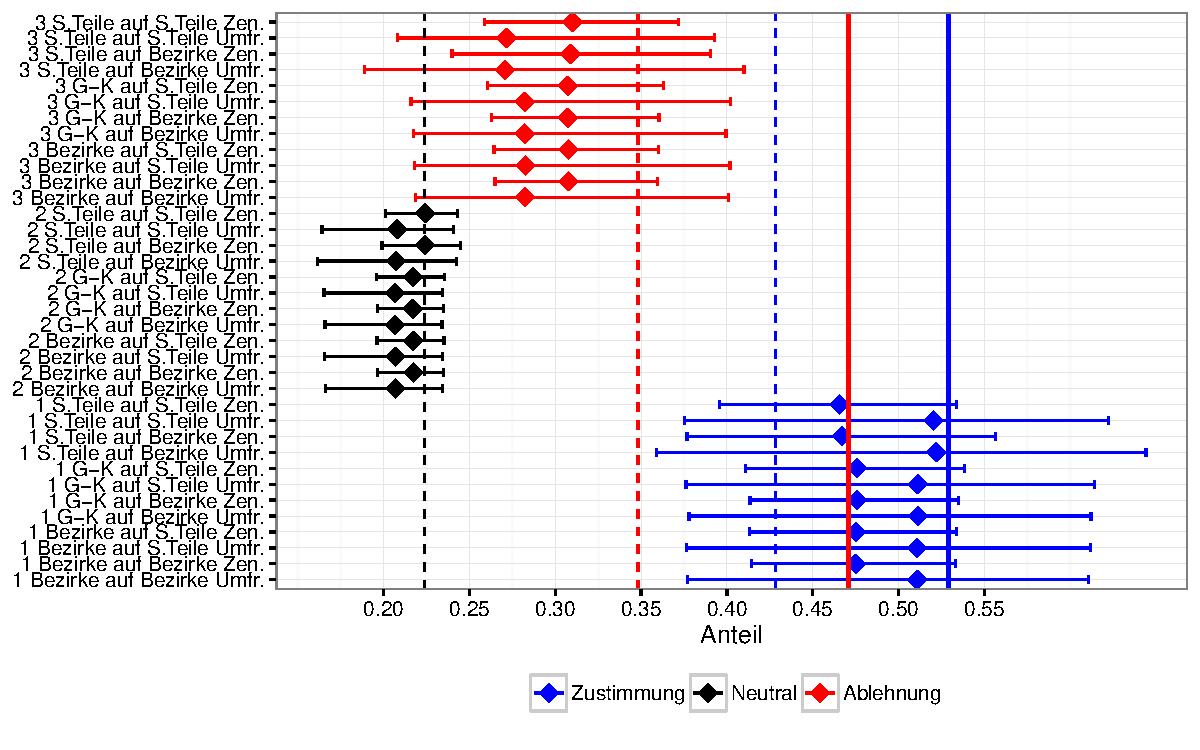
\includegraphics[scale=0.8]{Pictures/S21AlleModelle}
 \caption{Vergleich der extrapolierten Gesamtanteile für Stuttgart mit allen geschätzten Modellen und beiden Extrapolationsdateien mit den wahren Anteilen, sowie den Anteilen der Stichprobe mit 95\% Quantielen zur Meinung zu Stuttgart 21}
 \label{S21Alle}
 \end{center}
\end{figure}


\begin{figure}[h]
 \begin{center}
 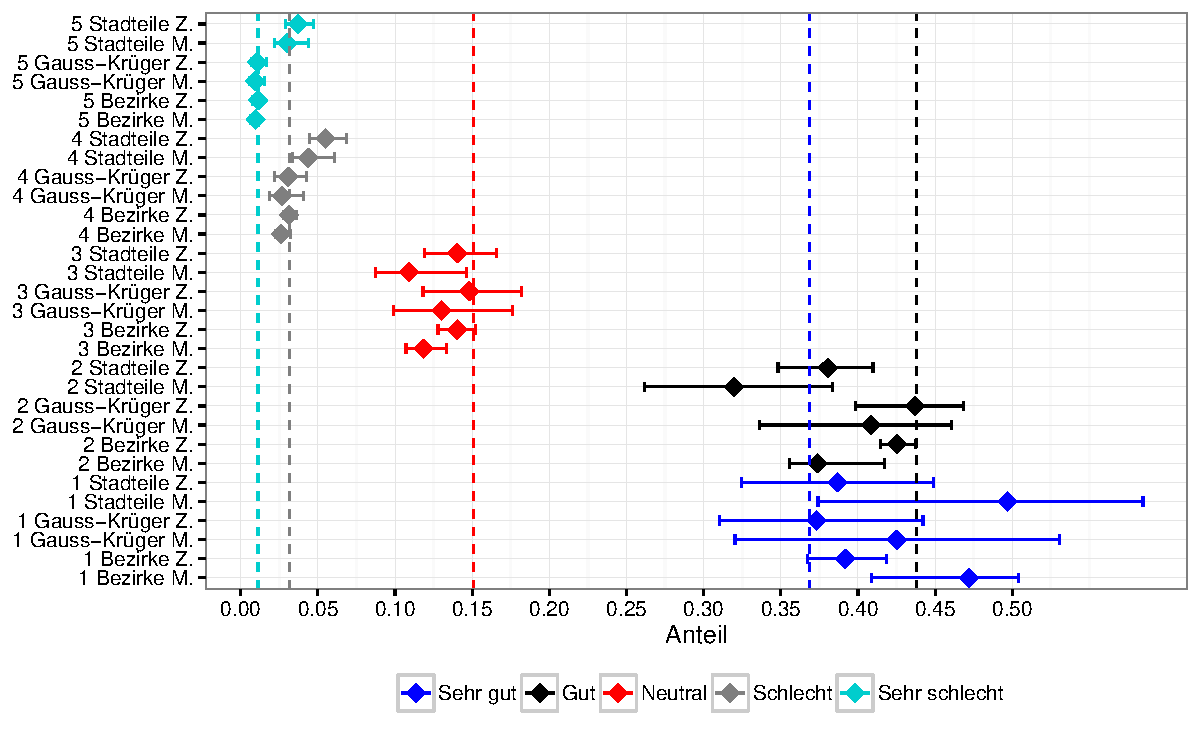
\includegraphics[scale=0.8]{Pictures/WohngegendAlleModelle2}
 \caption{Vergleich der extrapolierten Gesamtanteile für Stuttgart mit allen geschätzten Modellen und beiden Extrapolationsdateien mit den Anteilen der Stichprobe mit 95\% Quantielen zur Bewertung der Wohngegend}
 \label{WAlle}
 \end{center}
\end{figure}
%\clearpage

\section{Diskussion}
Die beiden Datensätze zur Grundgesamtheit stammen aus einer Melderegister mit 470.190 Beobachtungen und dem Zensus mit 380.238 Beobachtungen. Im Verhältnis zu den Grundgesamtheiten dieser Größenordnung sind 3143 Beobachtungen in der Stichprobe relativ gering, was eine gewisse Unsicherheit für die Extrapolation mit sich bringt [...].\\
Weiterhin ist zu beachten, dass Informationen zu dem monatlichen Netto Haushaltseinkommen in beiden Grundgesamtheiten fehlen und somit die Variable nicht für die Prognose verwendet werden kann. Auch war eine denkbare Erstellung von Proxy-Variablen nicht möglich. Eine genaue Auflistung der enthaltenen Variablen aus den Grundgesamtheiten ist im Anhang verfügbar. Die Arbeit zielt darauf ab, die Meinung der Befragten zu dem Projekt Stuttgart 21 und die Zufriedenheit mit der Wohngegend der Befragten auf die Grundgesamtheit zu extrapolieren. Daher ist es sinnvoll die Ausprägungen dieser Variablen genauer zu untersuchen.\\


Insgesamt ist zu sagen, dass die Gauss-Krüger Informationen ein relativ klaren Einblick in die Verteilung der Beobachtungen in der jeweiligen Klasse geben. Bei den diskreten räumlichen Informationen könnte die grobe Aufteilung auf Bezirksebene zu einem Underfitting und die sehr feine Aufteilung auf Stadtteilebene zu einem Overfitting führen [...]. Zudem ist zu vermuten, dass die räumlichen Informationen einen stärkeren Effekt auf die Bewertung der Wohngegend haben, als auf die Meinung zu Stuttgart 21.

Ein \textit{B} von 1.000 erwies sich als ausreichend, da sich die Mittelwerte und Quantile bei einer Erhöhung kaum noch änderten.

%============================================== Conlcusion =========================================================%

\section{Fazit}

\clearpage


%============================================ References ===========================================================%
\addcontentsline{toc}{section}{\numberline{}Literatur}
\bibliographystyle{apalike}
\bibliography{LiteraturStuttgart.bib} 

%\section{References}
%\renewcommand{\section}[2]{}
%\addcontentsline{toc}{section}{References}
%\renewcommand{\bibname}{4 References}
%\phantomsection
%\addcontentsline{toc}{section}{References}




\clearpage

%============================================== Appendix ============================================================%
%\appendix
%\pagestyle{Myheadings}
\chead{ANHANG}
%\pagestyle{}
%\section{$A^{-1}$ Appendix}
%\setcounter{secnumdepth}{0}

\begin{appendix}

\section*{Anhang}
\addcontentsline{toc}{section}{\numberline{}Anhang}






\begin{figure}[h]
 \begin{center}
 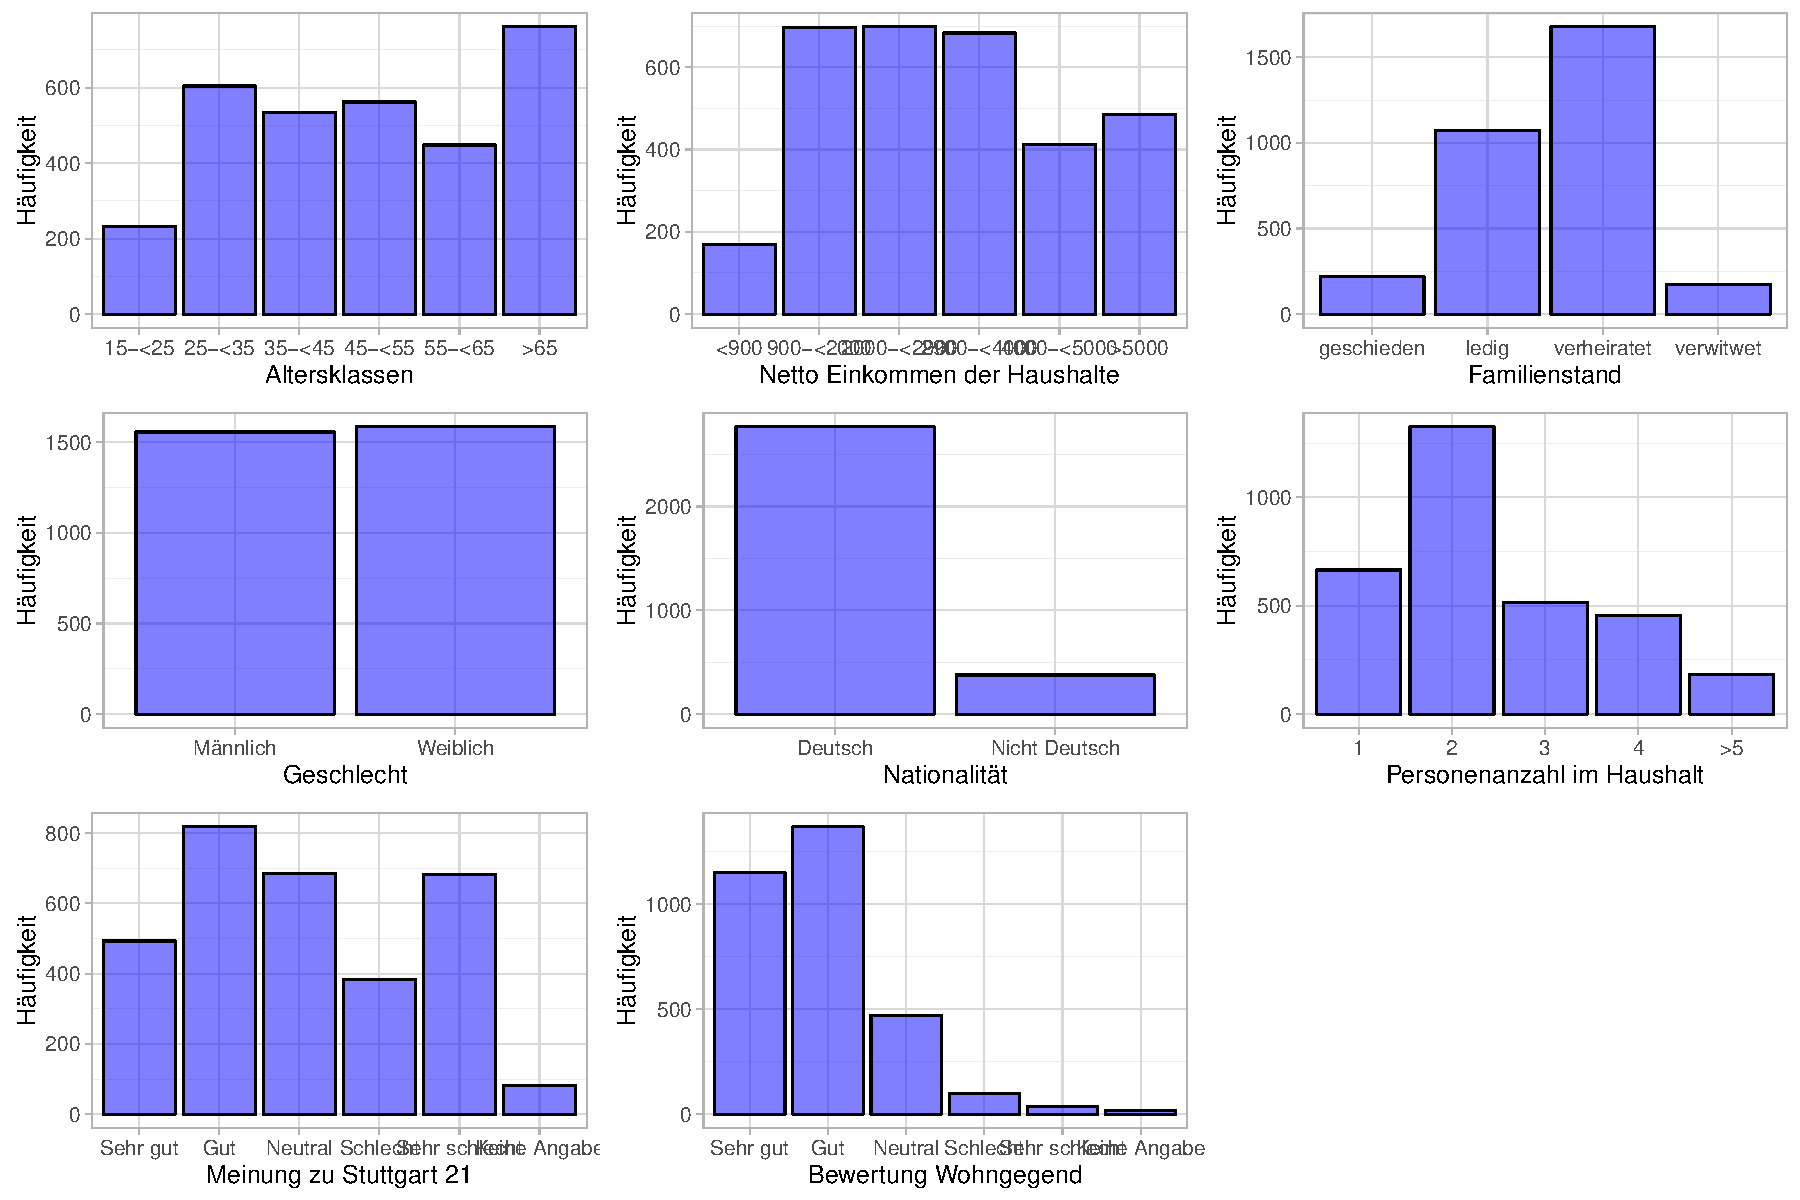
\includegraphics[scale=0.8]{Pictures/BarData}
 \caption{Häufigkeit der Kategorienausprägungen der exogenen Variablen in der Parameterisierungsstichprobe.}
 \label{exogen_parametrisierungsdatensatz}
 \end{center}
\end{figure}


\begin{figure}[h]
 \begin{center}
 
\includegraphics[scale=0.8]{Pictures/BWohn}
 \caption{Anteile der Bewertung der Wohngegend nach Stadtbezirken.}
 \label{BWohn}
 \end{center}
\end{figure}

\begin{figure}[h]
 \begin{center}
 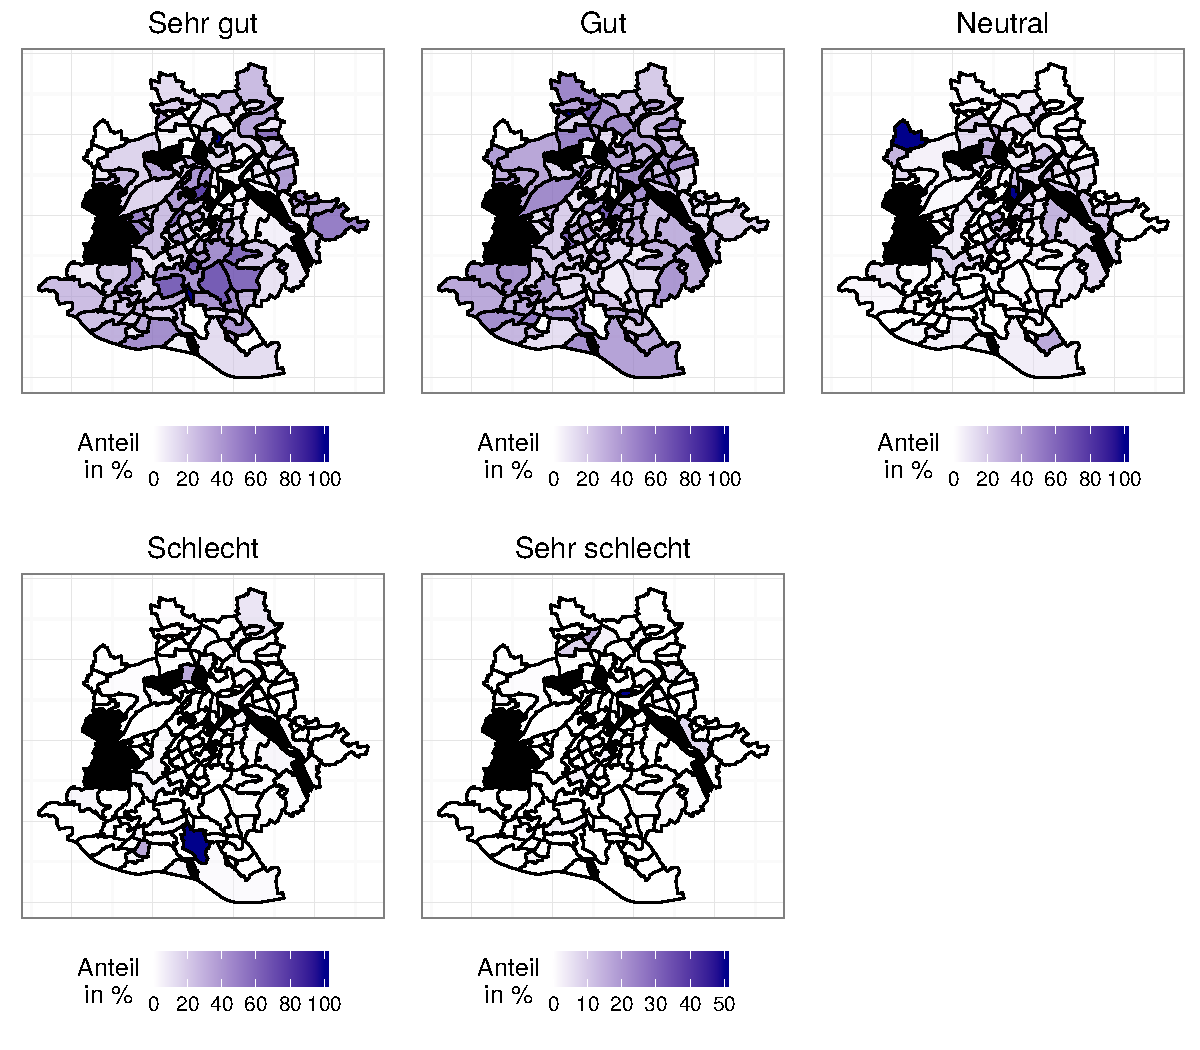
\includegraphics[scale=0.8]{Pictures/SWohn}
 \caption{Anteile der Bewertung der Wohngegend nach Stadtteilen.}
 \label{SWohn}
 \end{center}
\end{figure}

%\begin{figure}[h]
% \begin{center}
% 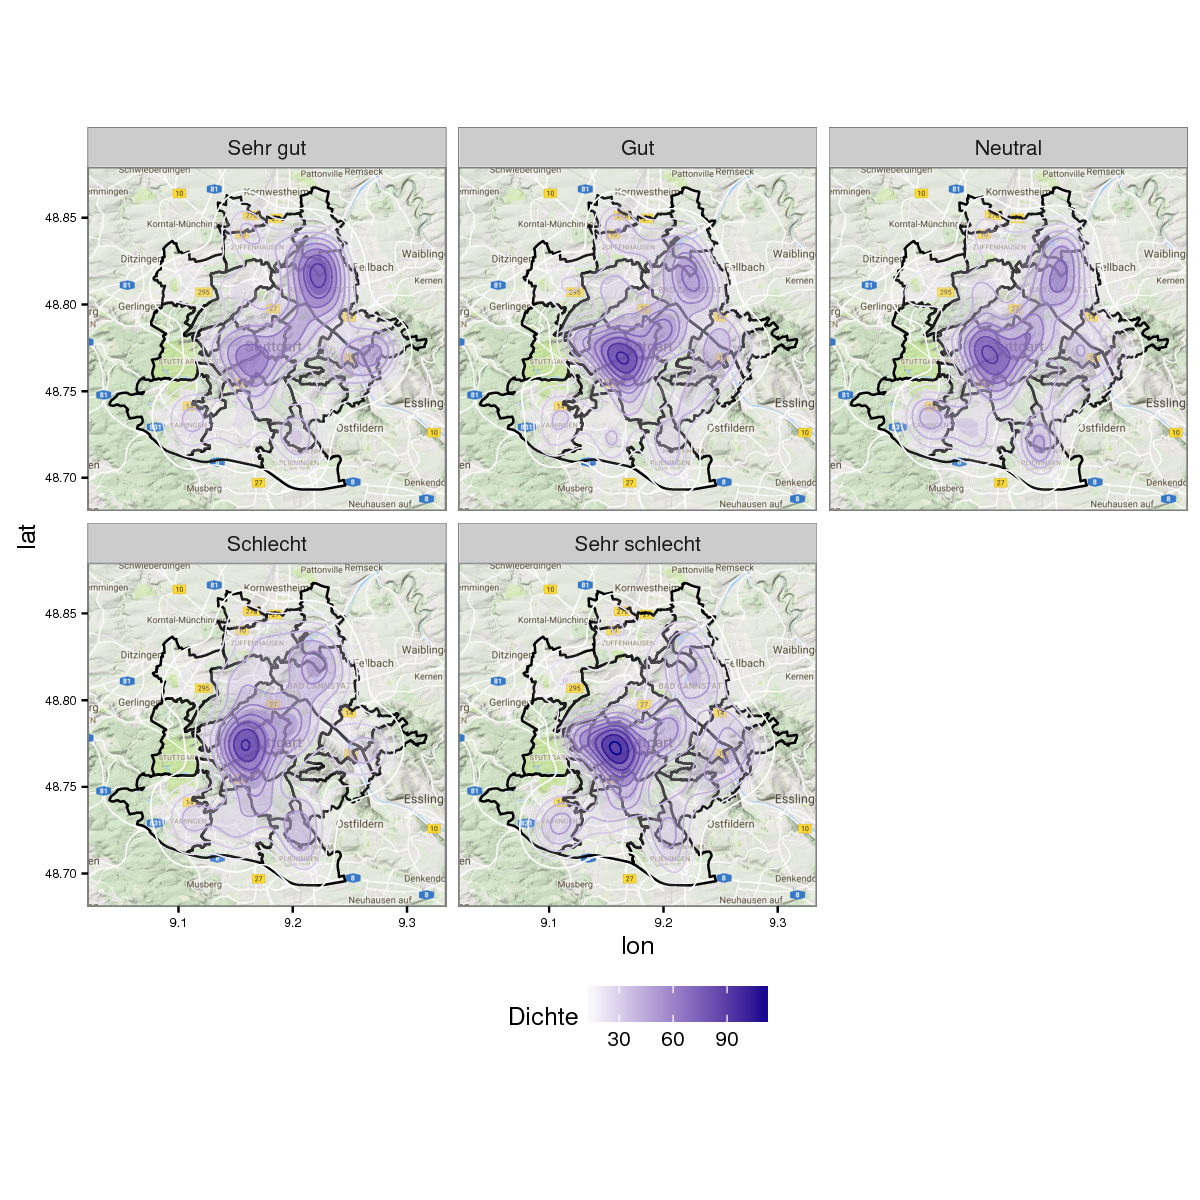
\includegraphics[scale=0.8]{Pictures/XYStuttgart5}
% \caption{Gauss Krüger Informationen Stuttgart 21 (2)}
% \label{endogene}
% \end{center}
%\end{figure}

\end{appendix}
\clearpage
\pagestyle{plain}
%\phantomsection
%\addcontentsline{toc}{section}{Eigenständigkeitserklärung}

%\section{Eigenständigkeitserklärung}

Hiermit versichere ich, dass ich die vorliegende Hausarbeit selbstständig verfasst und keine anderen als die angegebenen
Hilfsmittel benutzt habe. Alle wörtlich oder sinngemäß den Schriften anderer entnommenen Stellen
habe ich unter Angabe der Quellen kenntlich gemacht. Dies gilt auch für beigefügte Zeichnungen, Skizzen, bildliche
Darstellungen und dergleichen.\\
\\
Mir ist bewusst, dass ich mich im Falle einer unbeabsichtigten oder vorsätzlichen Missachtung durch den fehlerhaften
Umgang mit Quellen unter Umständen strafbar mache und die vorliegende Hausarbeit mit nicht ausreichend
bewertet wird.
\\
\\Göttingen, den
\\Unterschrift
\vspace*{4cm}
\\
Hiermit erlaube ich, dass meine Arbeit auf Betrug und falsche, sowie fehlende Zitate auch online geprüft wird.\\
\\
Mir ist bewusst, dass ich mich im Falle einer unbeabsichtigten oder vorsätzlichen Missachtung durch den fehlerhaften
Umgang mit Quellen unter Umständen strafbar mache und die vorliegende Hausarbeit mit nicht ausreichend
bewertet wird.
\\
\\Göttingen, den
\\Unterschrift
\clearpage


\end{document}
